% Options for packages loaded elsewhere
% Options for packages loaded elsewhere
\PassOptionsToPackage{unicode}{hyperref}
\PassOptionsToPackage{hyphens}{url}
%
\documentclass[
  ignorenonframetext,
  aspectratio=169,
]{beamer}
\newif\ifbibliography
\usepackage{pgfpages}
\setbeamertemplate{caption}[numbered]
\setbeamertemplate{caption label separator}{: }
\setbeamercolor{caption name}{fg=normal text.fg}
\beamertemplatenavigationsymbolsempty
% remove section numbering
\setbeamertemplate{part page}{
  \centering
  \begin{beamercolorbox}[sep=16pt,center]{part title}
    \usebeamerfont{part title}\insertpart\par
  \end{beamercolorbox}
}
\setbeamertemplate{section page}{
  \centering
  \begin{beamercolorbox}[sep=12pt,center]{section title}
    \usebeamerfont{section title}\insertsection\par
  \end{beamercolorbox}
}
\setbeamertemplate{subsection page}{
  \centering
  \begin{beamercolorbox}[sep=8pt,center]{subsection title}
    \usebeamerfont{subsection title}\insertsubsection\par
  \end{beamercolorbox}
}
% Prevent slide breaks in the middle of a paragraph
\widowpenalties 1 10000
\raggedbottom
\AtBeginPart{
  \frame{\partpage}
}
\AtBeginSection{
  \ifbibliography
  \else
    \frame{\sectionpage}
  \fi
}
\AtBeginSubsection{
  \frame{\subsectionpage}
}
\usepackage{iftex}
\ifPDFTeX
  \usepackage[T1]{fontenc}
  \usepackage[utf8]{inputenc}
  \usepackage{textcomp} % provide euro and other symbols
\else % if luatex or xetex
  \usepackage{unicode-math} % this also loads fontspec
  \defaultfontfeatures{Scale=MatchLowercase}
  \defaultfontfeatures[\rmfamily]{Ligatures=TeX,Scale=1}
\fi
\usepackage{lmodern}

\ifPDFTeX\else
  % xetex/luatex font selection
\fi
% Use upquote if available, for straight quotes in verbatim environments
\IfFileExists{upquote.sty}{\usepackage{upquote}}{}
\IfFileExists{microtype.sty}{% use microtype if available
  \usepackage[]{microtype}
  \UseMicrotypeSet[protrusion]{basicmath} % disable protrusion for tt fonts
}{}
\makeatletter
\@ifundefined{KOMAClassName}{% if non-KOMA class
  \IfFileExists{parskip.sty}{%
    \usepackage{parskip}
  }{% else
    \setlength{\parindent}{0pt}
    \setlength{\parskip}{6pt plus 2pt minus 1pt}}
}{% if KOMA class
  \KOMAoptions{parskip=half}}
\makeatother


\usepackage{longtable,booktabs,array}
\usepackage{calc} % for calculating minipage widths
\usepackage{caption}
% Make caption package work with longtable
\makeatletter
\def\fnum@table{\tablename~\thetable}
\makeatother
\usepackage{graphicx}
\makeatletter
\newsavebox\pandoc@box
\newcommand*\pandocbounded[1]{% scales image to fit in text height/width
  \sbox\pandoc@box{#1}%
  \Gscale@div\@tempa{\textheight}{\dimexpr\ht\pandoc@box+\dp\pandoc@box\relax}%
  \Gscale@div\@tempb{\linewidth}{\wd\pandoc@box}%
  \ifdim\@tempb\p@<\@tempa\p@\let\@tempa\@tempb\fi% select the smaller of both
  \ifdim\@tempa\p@<\p@\scalebox{\@tempa}{\usebox\pandoc@box}%
  \else\usebox{\pandoc@box}%
  \fi%
}
% Set default figure placement to htbp
\def\fps@figure{htbp}
\makeatother


% definitions for citeproc citations
\NewDocumentCommand\citeproctext{}{}
\NewDocumentCommand\citeproc{mm}{%
  \begingroup\def\citeproctext{#2}\cite{#1}\endgroup}
\makeatletter
 % allow citations to break across lines
 \let\@cite@ofmt\@firstofone
 % avoid brackets around text for \cite:
 \def\@biblabel#1{}
 \def\@cite#1#2{{#1\if@tempswa , #2\fi}}
\makeatother
\newlength{\cslhangindent}
\setlength{\cslhangindent}{1.5em}
\newlength{\csllabelwidth}
\setlength{\csllabelwidth}{3em}
\newenvironment{CSLReferences}[2] % #1 hanging-indent, #2 entry-spacing
 {\begin{list}{}{%
  \setlength{\itemindent}{0pt}
  \setlength{\leftmargin}{0pt}
  \setlength{\parsep}{0pt}
  % turn on hanging indent if param 1 is 1
  \ifodd #1
   \setlength{\leftmargin}{\cslhangindent}
   \setlength{\itemindent}{-1\cslhangindent}
  \fi
  % set entry spacing
  \setlength{\itemsep}{#2\baselineskip}}}
 {\end{list}}
\usepackage{calc}
\newcommand{\CSLBlock}[1]{\hfill\break\parbox[t]{\linewidth}{\strut\ignorespaces#1\strut}}
\newcommand{\CSLLeftMargin}[1]{\parbox[t]{\csllabelwidth}{\strut#1\strut}}
\newcommand{\CSLRightInline}[1]{\parbox[t]{\linewidth - \csllabelwidth}{\strut#1\strut}}
\newcommand{\CSLIndent}[1]{\hspace{\cslhangindent}#1}



\setlength{\emergencystretch}{3em} % prevent overfull lines

\providecommand{\tightlist}{%
  \setlength{\itemsep}{0pt}\setlength{\parskip}{0pt}}



 


\setkeys{Gin}{width=0.7\linewidth, keepaspectratio}
\makeatletter
\@ifpackageloaded{tcolorbox}{}{\usepackage[skins,breakable]{tcolorbox}}
\@ifpackageloaded{fontawesome5}{}{\usepackage{fontawesome5}}
\definecolor{quarto-callout-color}{HTML}{909090}
\definecolor{quarto-callout-note-color}{HTML}{0758E5}
\definecolor{quarto-callout-important-color}{HTML}{CC1914}
\definecolor{quarto-callout-warning-color}{HTML}{EB9113}
\definecolor{quarto-callout-tip-color}{HTML}{00A047}
\definecolor{quarto-callout-caution-color}{HTML}{FC5300}
\definecolor{quarto-callout-color-frame}{HTML}{acacac}
\definecolor{quarto-callout-note-color-frame}{HTML}{4582ec}
\definecolor{quarto-callout-important-color-frame}{HTML}{d9534f}
\definecolor{quarto-callout-warning-color-frame}{HTML}{f0ad4e}
\definecolor{quarto-callout-tip-color-frame}{HTML}{02b875}
\definecolor{quarto-callout-caution-color-frame}{HTML}{fd7e14}
\makeatother
\makeatletter
\@ifpackageloaded{caption}{}{\usepackage{caption}}
\AtBeginDocument{%
\ifdefined\contentsname
  \renewcommand*\contentsname{Table of contents}
\else
  \newcommand\contentsname{Table of contents}
\fi
\ifdefined\listfigurename
  \renewcommand*\listfigurename{List of Figures}
\else
  \newcommand\listfigurename{List of Figures}
\fi
\ifdefined\listtablename
  \renewcommand*\listtablename{List of Tables}
\else
  \newcommand\listtablename{List of Tables}
\fi
\ifdefined\figurename
  \renewcommand*\figurename{Figure}
\else
  \newcommand\figurename{Figure}
\fi
\ifdefined\tablename
  \renewcommand*\tablename{Table}
\else
  \newcommand\tablename{Table}
\fi
}
\@ifpackageloaded{float}{}{\usepackage{float}}
\floatstyle{ruled}
\@ifundefined{c@chapter}{\newfloat{codelisting}{h}{lop}}{\newfloat{codelisting}{h}{lop}[chapter]}
\floatname{codelisting}{Listing}
\newcommand*\listoflistings{\listof{codelisting}{List of Listings}}
\makeatother
\makeatletter
\makeatother
\makeatletter
\@ifpackageloaded{caption}{}{\usepackage{caption}}
\@ifpackageloaded{subcaption}{}{\usepackage{subcaption}}
\makeatother

\usepackage{bookmark}
\IfFileExists{xurl.sty}{\usepackage{xurl}}{} % add URL line breaks if available
\urlstyle{same}
\hypersetup{
  pdftitle={Conceitos Iniciais},
  hidelinks,
  pdfcreator={LaTeX via pandoc}}



\title{Conceitos Iniciais}
\author{}
\date{}

\begin{document}
\frame{\titlepage}


\section{Motivação}\label{motivauxe7uxe3o}

\begin{frame}{Motivação}
\phantomsection\label{motivauxe7uxe3o-1}
\begin{columns}[T]
\begin{column}{0.5\linewidth}
\begin{quote}
``Nós estamos nos afogando em informação, mas sedentos por
conhecimento''.
\end{quote}

Naisbitt (1982)
\end{column}

\begin{column}{0.5\linewidth}
\begin{center}
\pandocbounded{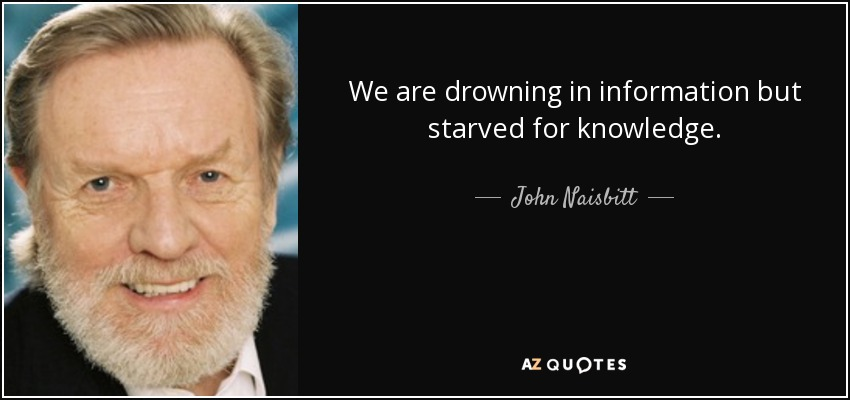
\includegraphics[keepaspectratio]{../../images/naisb.jpg}}
\end{center}
\end{column}
\end{columns}

\href{https://www.economist.com/leaders/2017/05/06/the-worlds-most-valuable-resource-is-no-longer-oil-but-data}{São
os dados, o novo petróleo?}
\end{frame}

\begin{frame}{Muitos dados, pouco conhecimento!}
\phantomsection\label{muitos-dados-pouco-conhecimento}
A quantidade de dados gerados diariamente vem \textbf{aumentando
exponencialmente}, tornando a análise de dados cada vez mais importante

\begin{figure}[H]

{\centering \pandocbounded{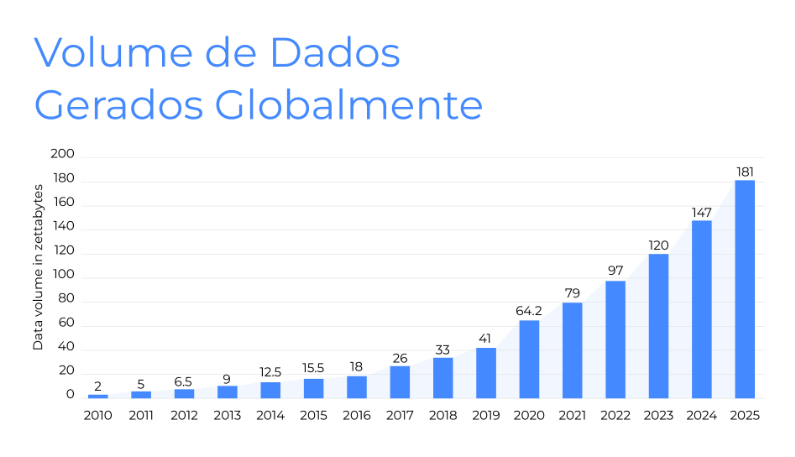
\includegraphics[keepaspectratio]{../../images/graf_dados.png}}

}

\caption{Fonte: statista}

\end{figure}%

👉 \textbf{Um zettabyte} é igual a \textbf{1 trilhão de gigabytes} 😲
\end{frame}

\begin{frame}{Muitos dados, pouco conhecimento!}
\phantomsection\label{muitos-dados-pouco-conhecimento-1}

\includegraphics[width=0.7\linewidth,height=\textheight,keepaspectratio]{../../images/data_every_where.png}
\end{frame}

\begin{frame}{Como usar o conhecimento?}
\phantomsection\label{como-usar-o-conhecimento}
\begin{center}
\pandocbounded{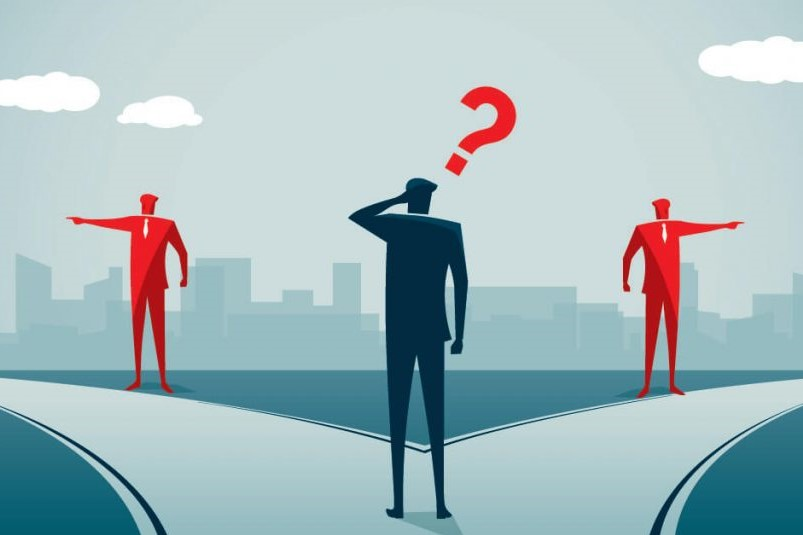
\includegraphics[keepaspectratio]{../../images/neg.jpg}}
\end{center}
\end{frame}

\begin{frame}{Como usar o conhecimento?}
\phantomsection\label{como-usar-o-conhecimento-1}
\begin{center}
\pandocbounded{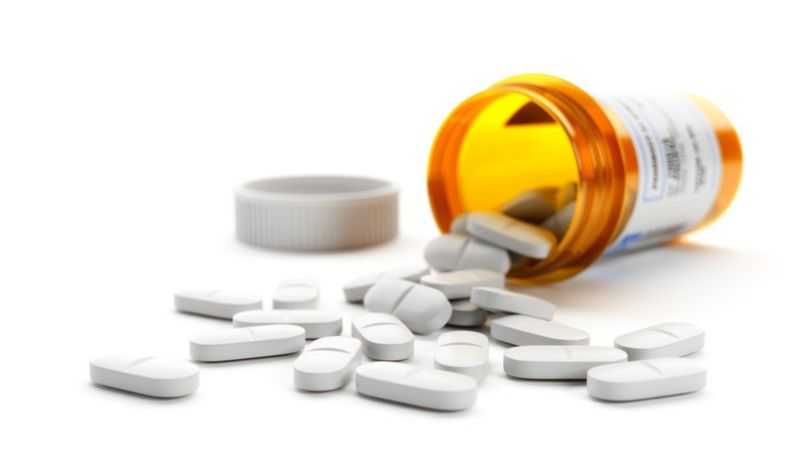
\includegraphics[keepaspectratio]{../../images/med.jpg}}
\end{center}
\end{frame}

\begin{frame}{Como usar o conhecimento?}
\phantomsection\label{como-usar-o-conhecimento-2}
\begin{center}
\pandocbounded{
\includegraphics[keepaspectratio]{../../images/crimes.jpg}}
\end{center}
\end{frame}

\begin{frame}{Como usar o conhecimento?}
\phantomsection\label{como-usar-o-conhecimento-3}
\begin{center}
\pandocbounded{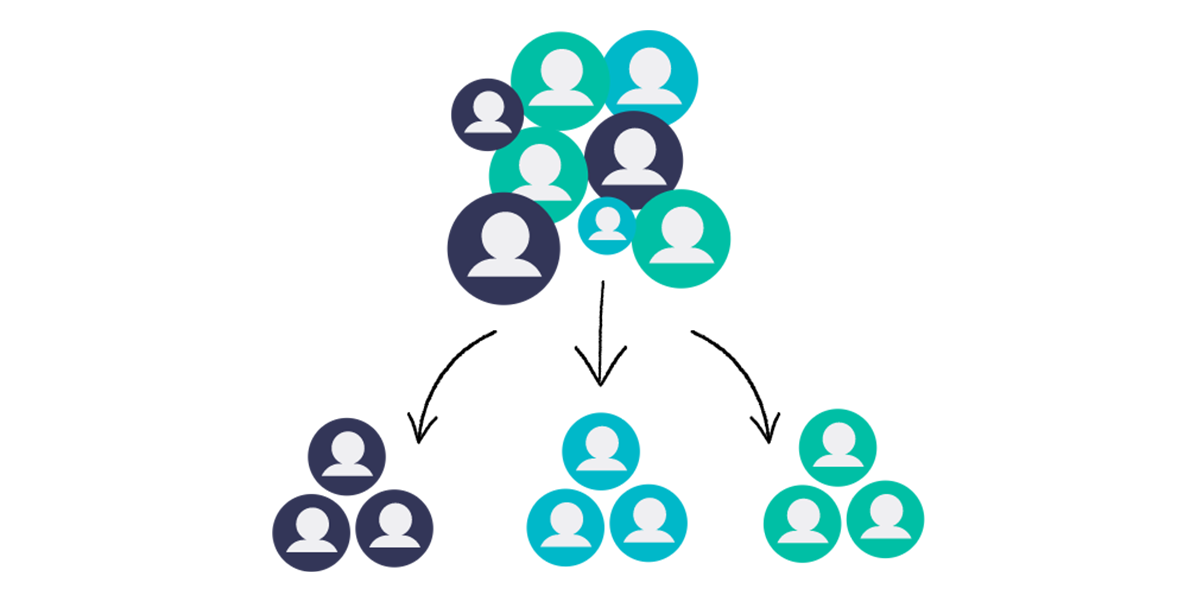
\includegraphics[keepaspectratio]{../../images/cliente.png}}
\end{center}
\end{frame}

\begin{frame}{O que é mineração de dados?}
\phantomsection\label{o-que-uxe9-minerauxe7uxe3o-de-dados}
\begin{columns}[T]
\begin{column}{0.5\linewidth}
A \textbf{mineração de dados} é o processo de descobrir
\textbf{conhecimentos ocultos} e \textbf{padrões} em \textbf{grandes
volumes} de dados.

Tem como \textbf{objetivo} transformar \textbf{dados brutos} em
\textbf{informações úteis} e \textbf{conhecimentos} para a
\textbf{tomada de decisão}.
\end{column}

\begin{column}{0.5\linewidth}
\begin{center}
\pandocbounded{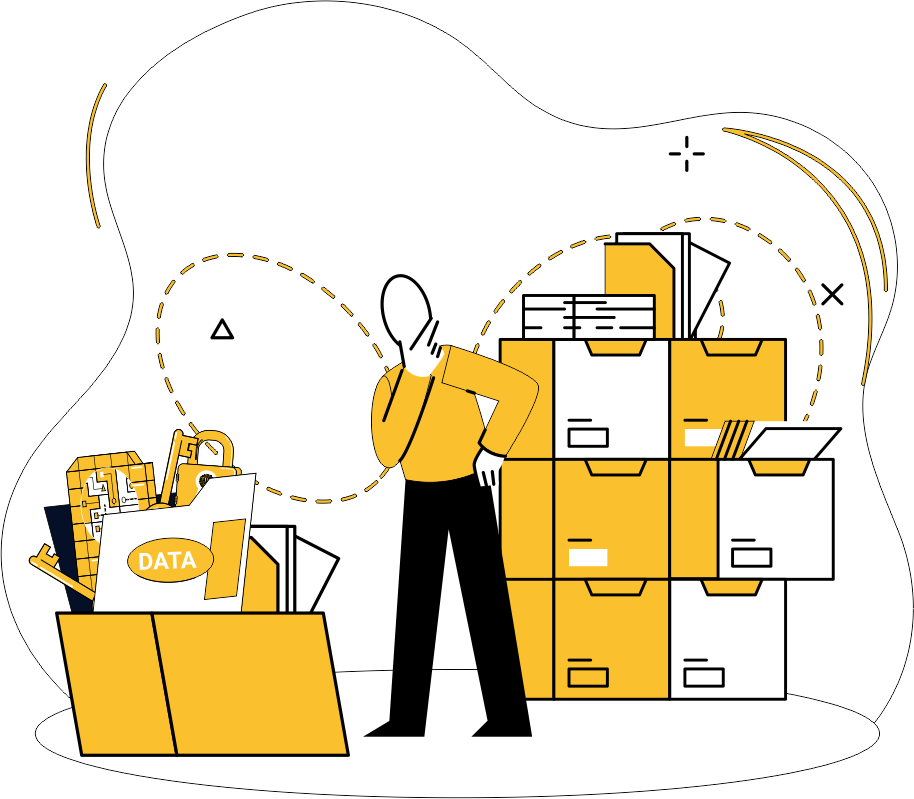
\includegraphics[keepaspectratio]{../../images/dados_em_conhecimento.png}}
\end{center}
\end{column}
\end{columns}
\end{frame}

\begin{frame}{O que é mineração de dados?}
\phantomsection\label{o-que-uxe9-minerauxe7uxe3o-de-dados-1}
\begin{columns}[T]
\begin{column}{0.5\linewidth}
\begin{center}
\pandocbounded{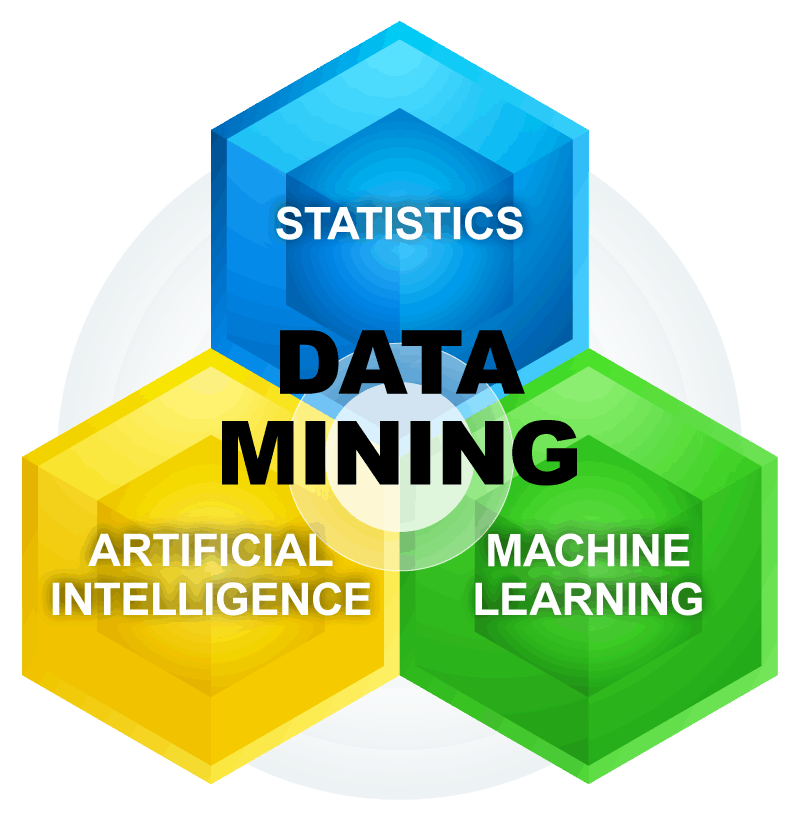
\includegraphics[keepaspectratio]{../../images/data_mining.png}}
\end{center}
\end{column}

\begin{column}{0.5\linewidth}
Ela usa técnicas de \textbf{aprendizado de máquina},
\textbf{estatística} e \textbf{inteligência artificial} para
\textbf{analisar dados} e extrair \textbf{insights}.

Essas técnicas transformam, de maneira inteligente e automática, os
\textbf{dados} disponíveis em \textbf{informações} úteis, que
representem o \textbf{conhecimento} para ser usado com
\textbf{sabedoria}.
\end{column}
\end{columns}
\end{frame}

\begin{frame}{Dado, informação, conhecimento e sabedoria}
\phantomsection\label{dado-informauxe7uxe3o-conhecimento-e-sabedoria}
\begin{columns}[T]
\begin{column}{0.5\linewidth}
\begin{center}
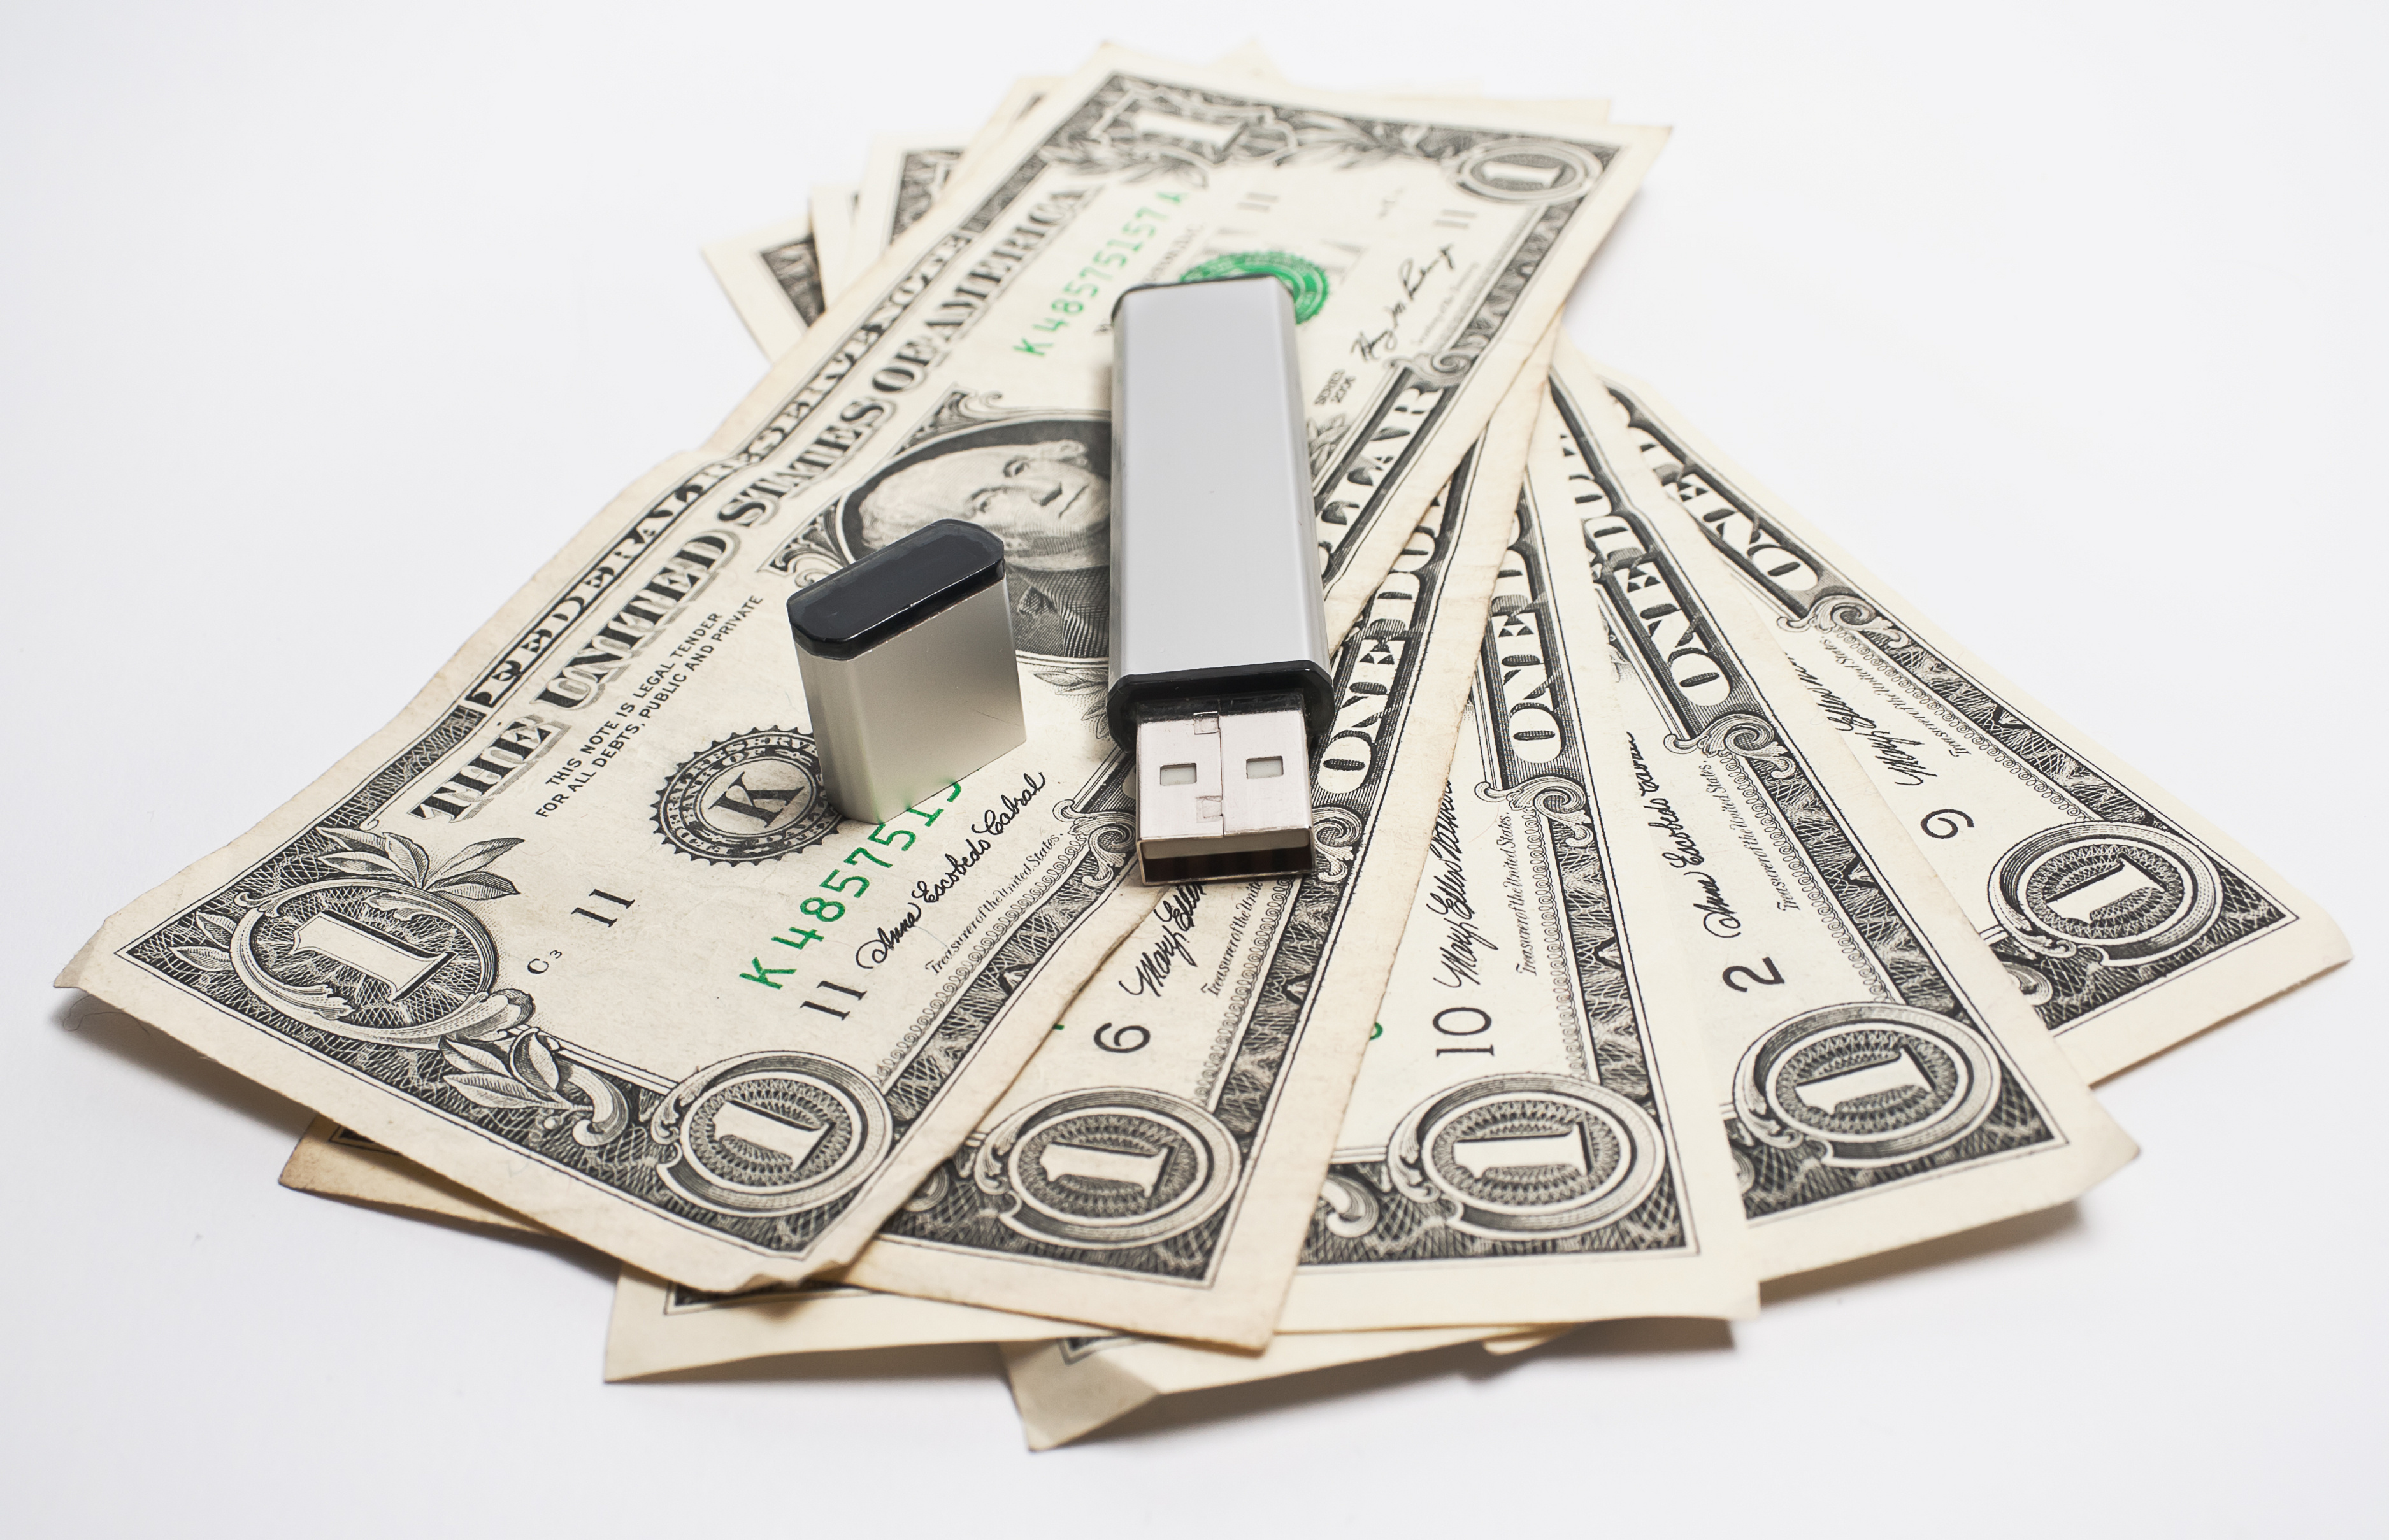
\includegraphics[width=8.33333in,height=\textheight,keepaspectratio]{../../images/info_dinheiro.png}
\end{center}
\end{column}

\begin{column}{0.5\linewidth}
\textbf{Informação}, e não \textbf{dados}, valem dinheiro, tempo,
conhecimento!
\end{column}
\end{columns}
\end{frame}

\begin{frame}{Dado, informação, conhecimento e sabedoria}
\phantomsection\label{dado-informauxe7uxe3o-conhecimento-e-sabedoria-1}
\begin{columns}[T]
\begin{column}{0.5\linewidth}
\begin{center}
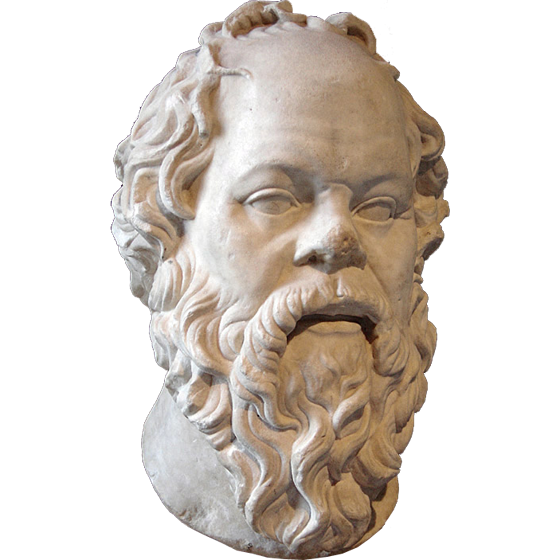
\includegraphics[width=8.33333in,height=\textheight,keepaspectratio]{../../images/socrates.png}
\end{center}
\end{column}

\begin{column}{0.5\linewidth}
Sócrates
\end{column}
\end{columns}
\end{frame}

\begin{frame}{Dado, informação, conhecimento e sabedoria}
\phantomsection\label{dado-informauxe7uxe3o-conhecimento-e-sabedoria-2}
\textbf{Dado:} são fatos brutos, sem significado ou contexto, que podem
ser registrados e armazenados.

\pause

\begin{center}

\includegraphics[width=7.29167in,height=\textheight,keepaspectratio]{../../images/dados.png}
\end{center}
\end{frame}

\begin{frame}{Dado, informação, conhecimento e sabedoria}
\phantomsection\label{dado-informauxe7uxe3o-conhecimento-e-sabedoria-3}
\textbf{Informação:} é o resultado da organização e interpretação dos
dados, dando-lhes significado e contexto.

\pause

\begin{center}
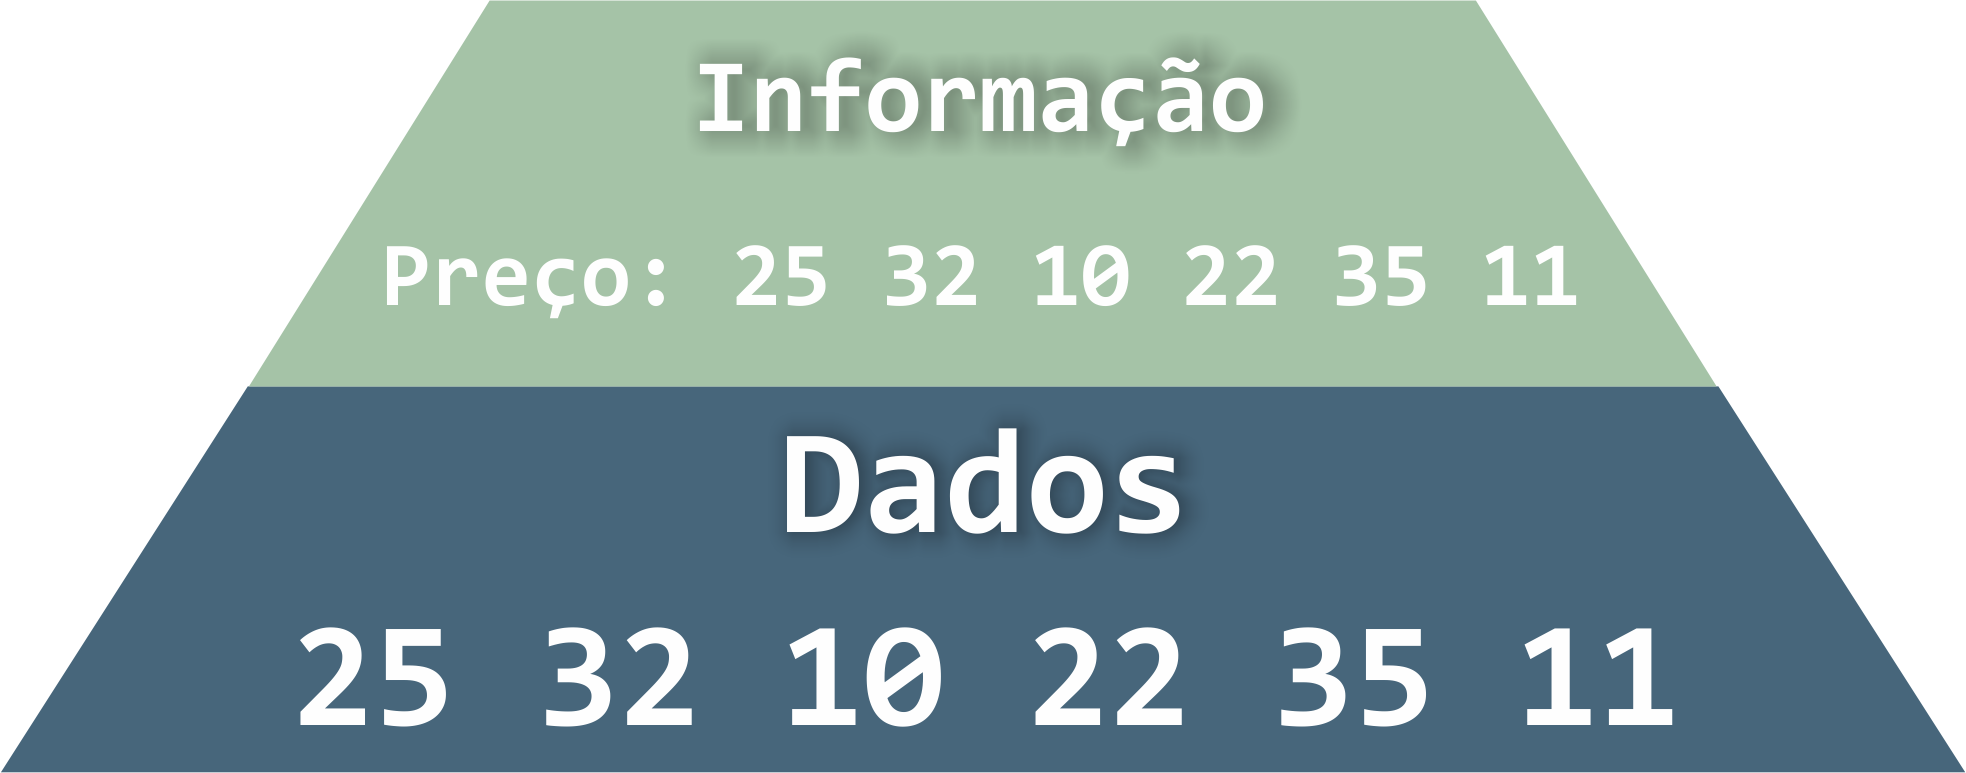
\includegraphics[width=7.29167in,height=\textheight,keepaspectratio]{../../images/info.png}
\end{center}
\end{frame}

\begin{frame}{Dado, informação, conhecimento e sabedoria}
\phantomsection\label{dado-informauxe7uxe3o-conhecimento-e-sabedoria-4}
\textbf{Conhecimento:} é a compreensão dos relacionamentos entre as
informações e a capacidade de aplicar essas informações em uma situação
específica.

\pause

\begin{center}
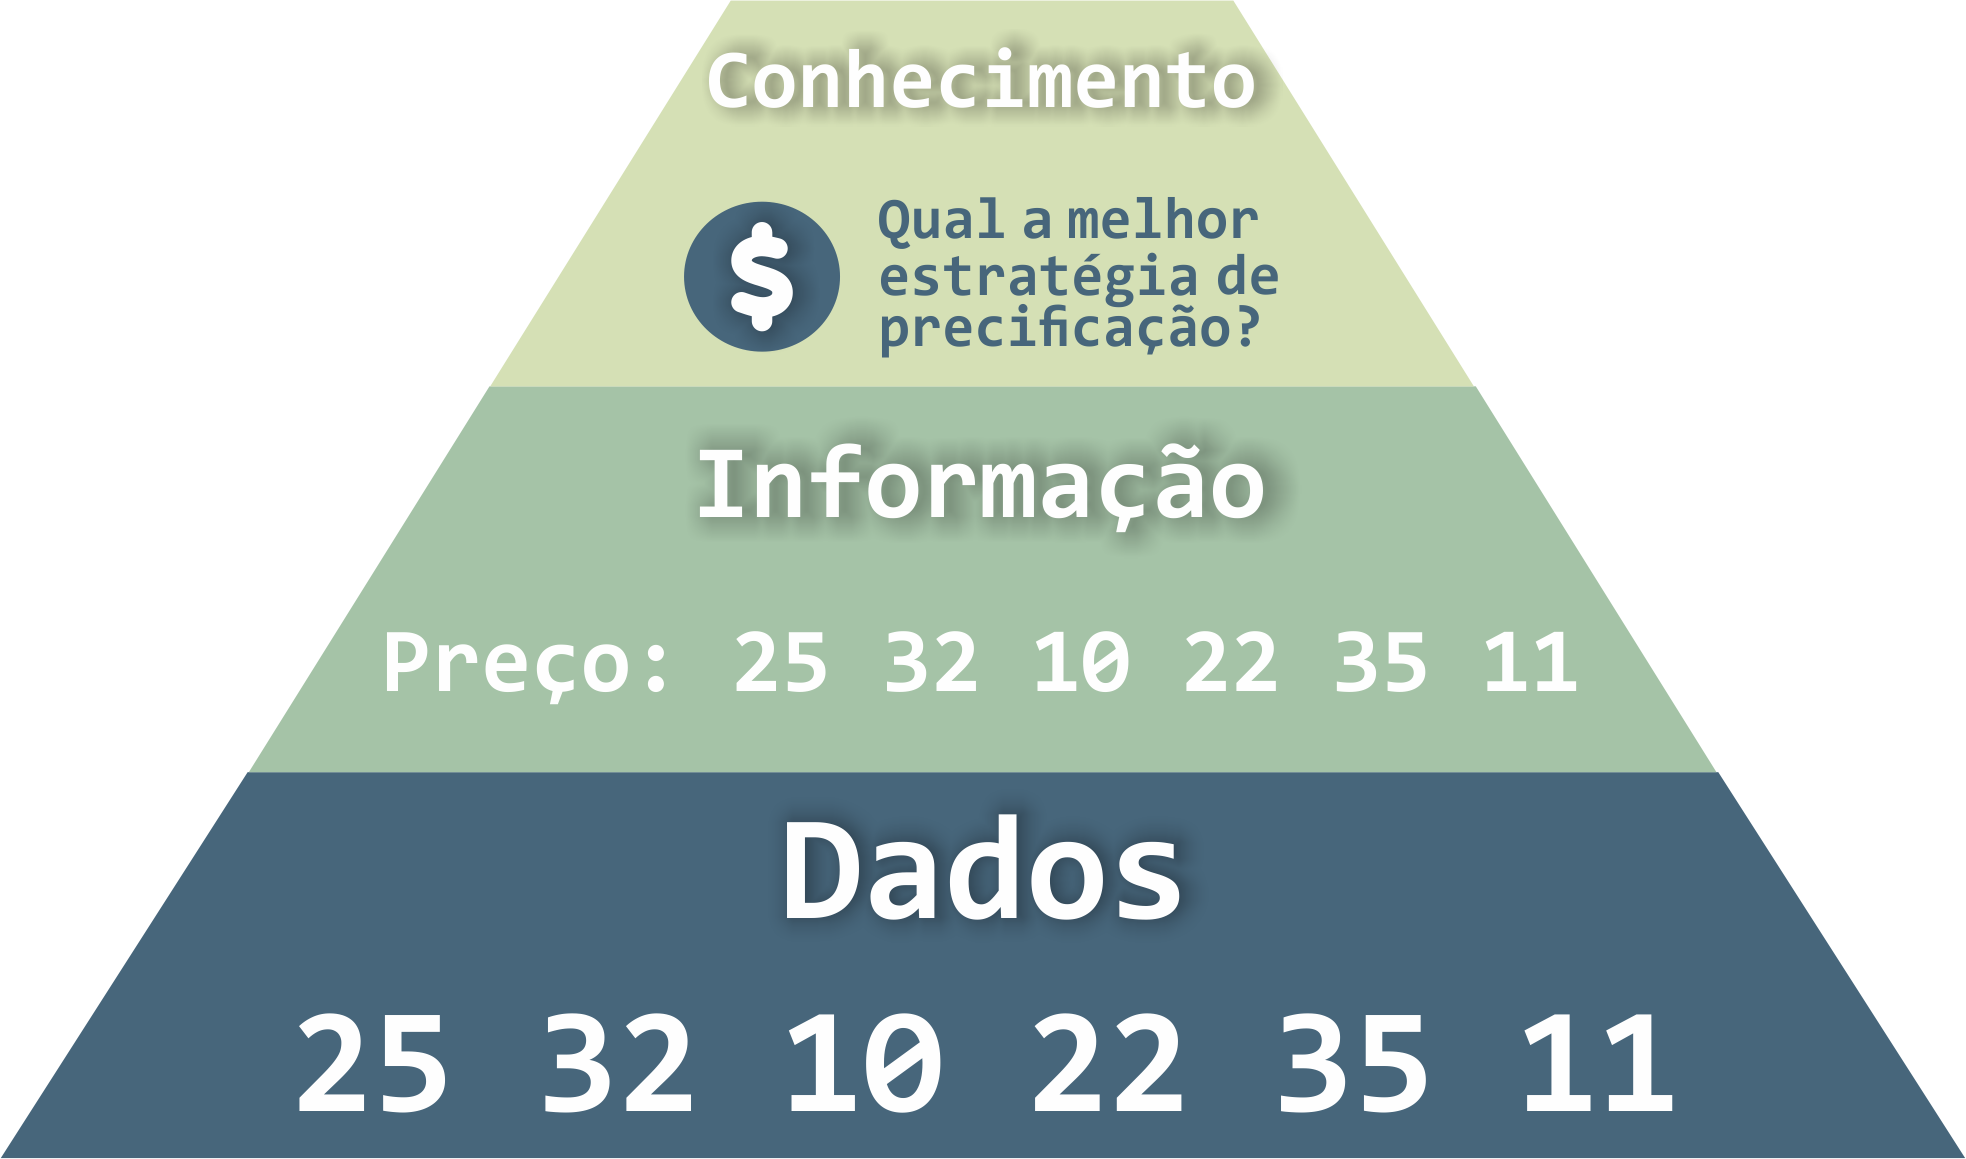
\includegraphics[width=7.29167in,height=\textheight,keepaspectratio]{../../images/conhecimento.png}
\end{center}
\end{frame}

\begin{frame}{Dado, informação, conhecimento e sabedoria}
\phantomsection\label{dado-informauxe7uxe3o-conhecimento-e-sabedoria-5}
\textbf{Sabedoria:} é a habilidade de usar o conhecimento de forma ética
e eficaz para tomar decisões sábias.

\pause

\begin{center}
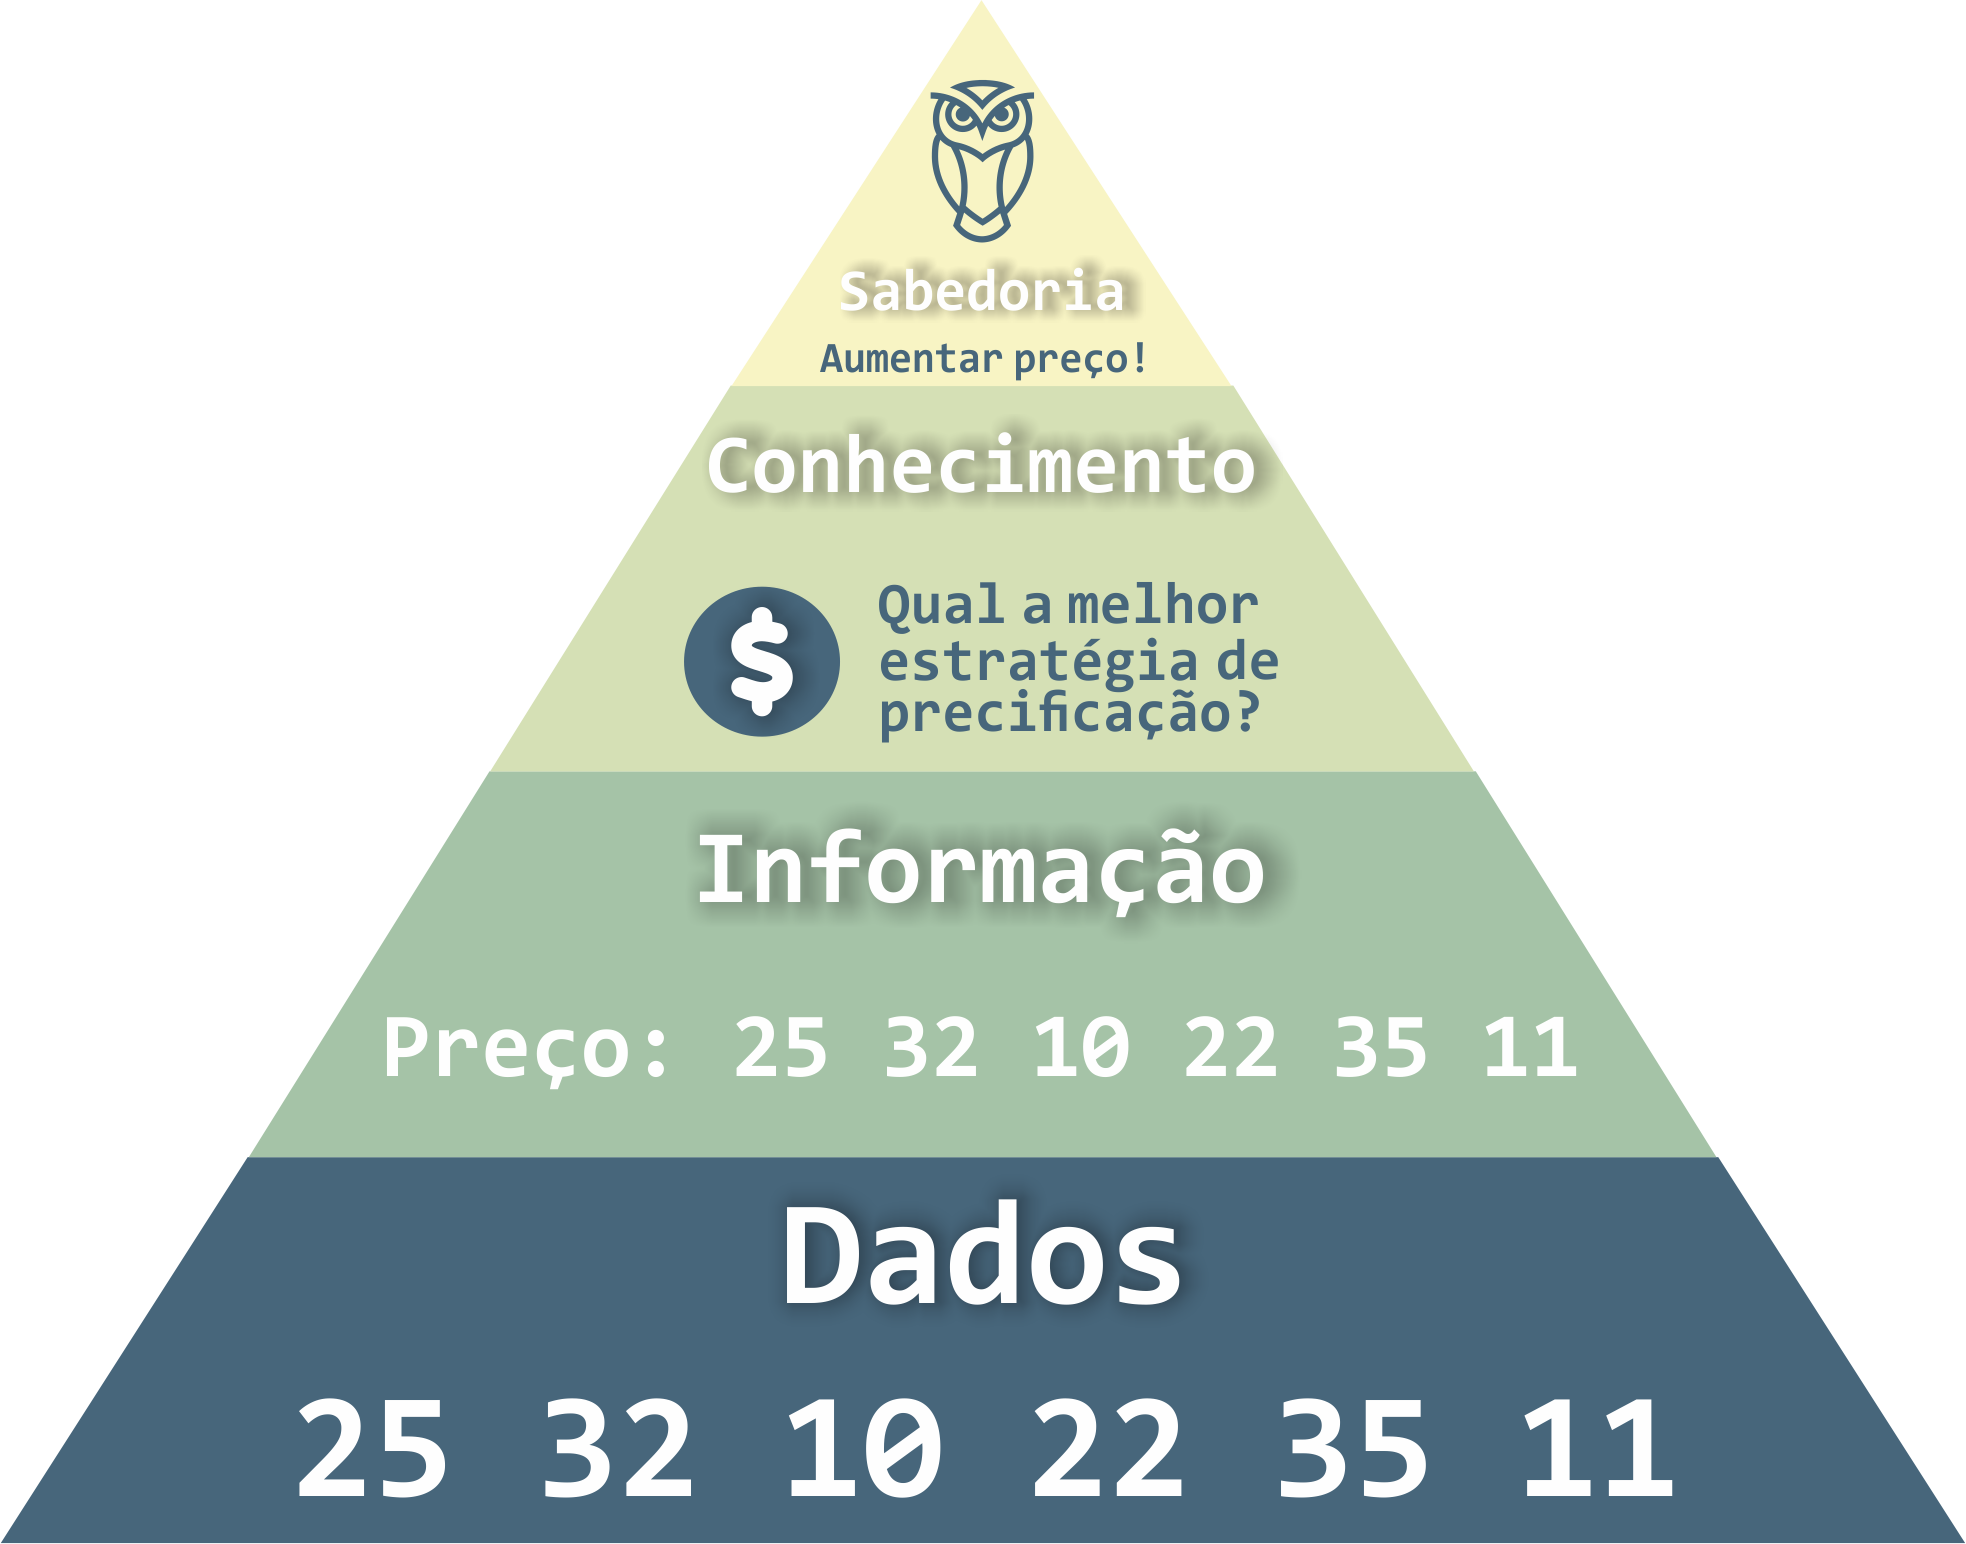
\includegraphics[width=7.29167in,height=\textheight,keepaspectratio]{../../images/sabedoria.png}
\end{center}
\end{frame}

\begin{frame}{CRISP-DM, SEMMA e KDD}
\phantomsection\label{crisp-dm-semma-e-kdd}
\begin{itemize}
\tightlist
\item
  \textbf{Gerenciamento de projetos} é um campo estabelecido focado no
  planejamento, entrega, controle e monitoramento de um projeto.
\end{itemize}

\pause

\begin{itemize}
\tightlist
\item
  Existem várias metodologias para gerenciar projetos de mineração de
  dados.
\end{itemize}

\pause

\begin{itemize}
\tightlist
\item
  Três das metodologias mais comuns são \textbf{CRISP-DM},
  \textbf{SEMMA} e \textbf{KDD}.
\end{itemize}
\end{frame}

\begin{frame}{KDD}
\phantomsection\label{kdd}
\begin{itemize}
\tightlist
\item
  KDD (\textbf{K}nowledge \textbf{D}iscovery in \textbf{D}atabases) é
  uma metodologia mais ampla que CRISP-DM e SEMMA.
\end{itemize}

\pause

\begin{itemize}
\item
  Envolve basicamente \textbf{três etapas}: pré-processamento, mineração
  de dados e pós-processamento.

  \begin{itemize}
  \tightlist
  \item
    \textbf{Pré-processamento} inclui limpeza, integração e
    transformação de dados.
  \item
    A \textbf{mineração de dados} inclui seleção, pré-processamento e
    modelagem de dados.
  \item
    O \textbf{pós-processamento} inclui interpretação e avaliação dos
    resultados.
  \end{itemize}
\end{itemize}
\end{frame}

\begin{frame}{KDD}
\phantomsection\label{kdd-1}
\begin{center}
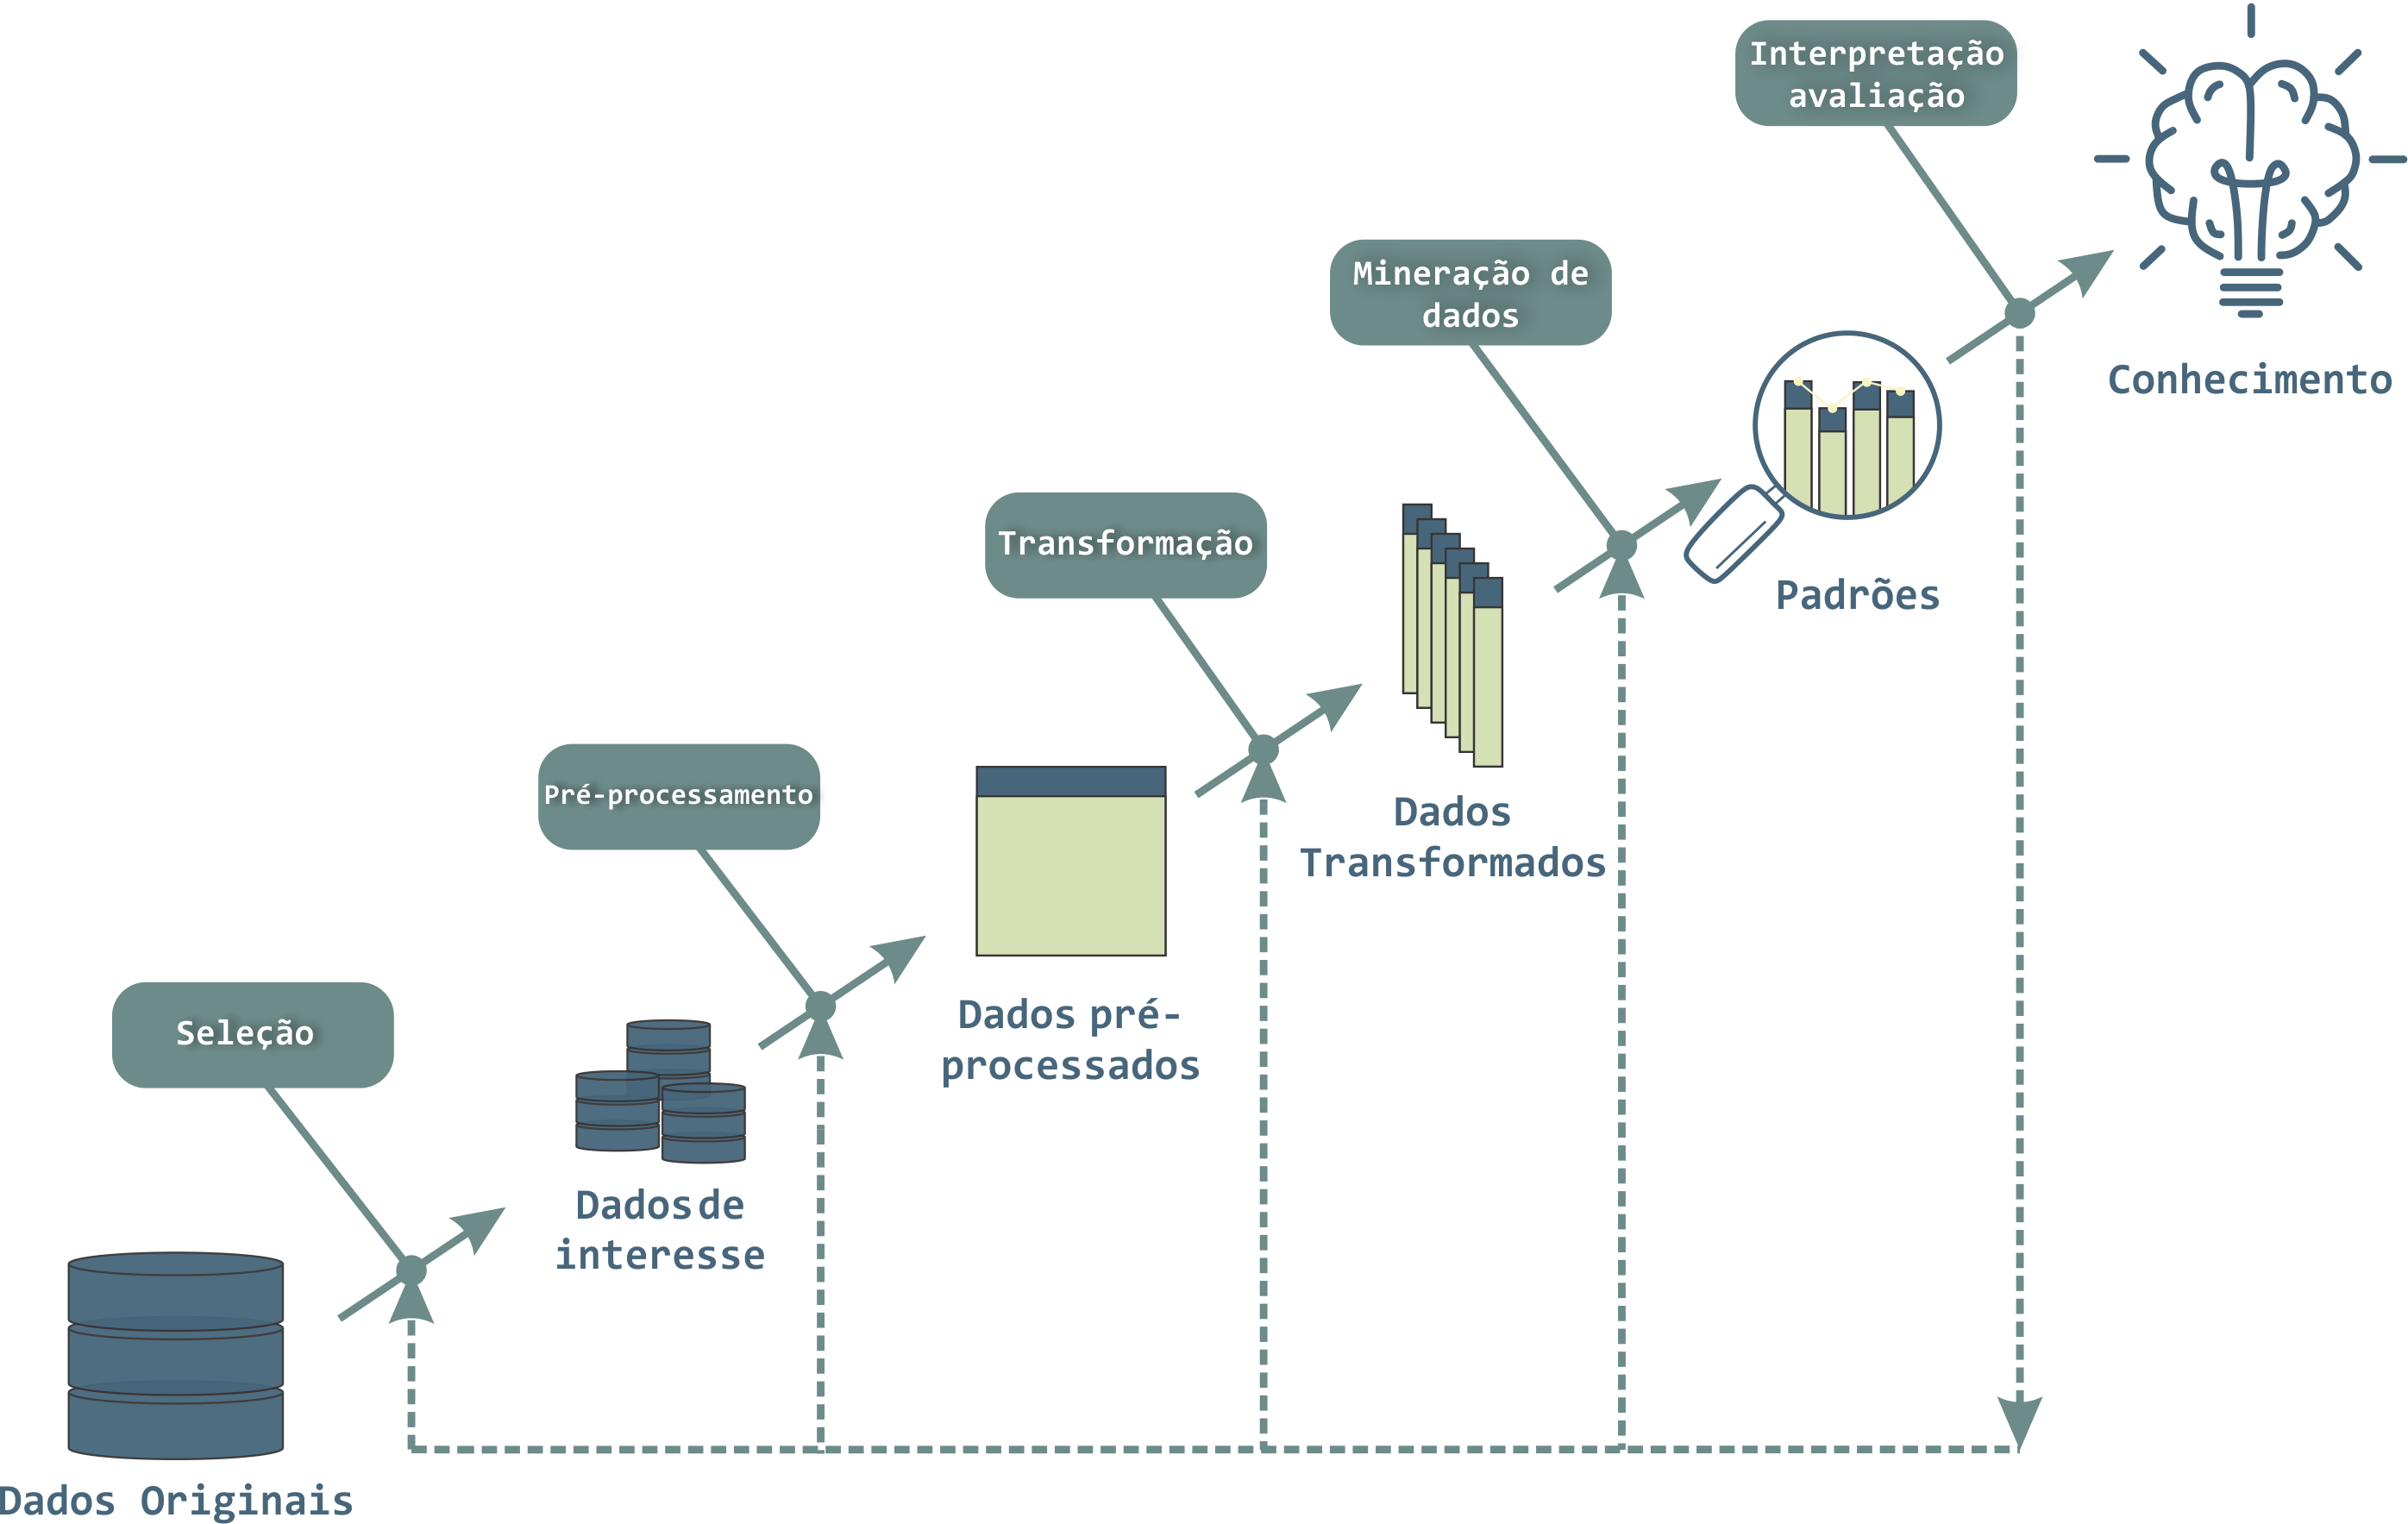
\includegraphics[width=7.29167in,height=\textheight,keepaspectratio]{../../images/kdd.png}
\end{center}
\end{frame}

\begin{frame}{KDD: Seleção}
\phantomsection\label{kdd-seleuxe7uxe3o}
\begin{itemize}
\tightlist
\item
  Nesta fase, o objetivo é selecionar os dados relevantes para o
  problema de mineração.
\end{itemize}

\pause

\begin{itemize}
\tightlist
\item
  É importante identificar as fontes de dados relevantes e escolher as
  variáveis de interesse.
\end{itemize}
\end{frame}

\begin{frame}{KDD: Pré-processamento}
\phantomsection\label{kdd-pruxe9-processamento}
\begin{itemize}
\tightlist
\item
  Nesta fase, o objetivo é preparar os dados para análise.
\end{itemize}

\pause

\begin{itemize}
\tightlist
\item
  É importante lidar com valores ausentes, tratar outliers e realizar
  normalização ou padronização de variáveis.
\end{itemize}
\end{frame}

\begin{frame}{KDD: Limpeza}
\phantomsection\label{kdd-limpeza}
\begin{itemize}
\tightlist
\item
  Nesta fase, o objetivo é identificar e corrigir erros nos dados.
\end{itemize}

\pause

\begin{itemize}
\tightlist
\item
  É importante lidar com dados duplicados, corrigir erros de digitação e
  identificar e tratar valores discrepantes.
\end{itemize}
\end{frame}

\begin{frame}{KDD: Transformação}
\phantomsection\label{kdd-transformauxe7uxe3o}
\begin{itemize}
\tightlist
\item
  Nesta fase, o objetivo é transformar os dados em uma forma que seja
  adequada para a análise.
\end{itemize}

\pause

\begin{itemize}
\tightlist
\item
  É importante realizar transformações como discretização, agregação, e
  normalização para que os dados possam ser usados com sucesso na
  modelagem.
\end{itemize}
\end{frame}

\begin{frame}{KDD: Mineração de dados}
\phantomsection\label{kdd-minerauxe7uxe3o-de-dados}
\begin{itemize}
\tightlist
\item
  Nesta fase, o objetivo é aplicar técnicas de mineração de dados para
  identificar padrões e relacionamentos nos dados.
\end{itemize}

\pause

\begin{itemize}
\tightlist
\item
  É importante escolher as técnicas de mineração de dados apropriadas e
  avaliar a eficácia dos modelos gerados.
\end{itemize}
\end{frame}

\begin{frame}{KDD: Interpretação e avaliação}
\phantomsection\label{kdd-interpretauxe7uxe3o-e-avaliauxe7uxe3o}
\begin{itemize}
\tightlist
\item
  Nesta fase, o objetivo é interpretar os resultados da mineração de
  dados e avaliar sua relevância para o problema de negócio.
\end{itemize}

\pause

\begin{itemize}
\tightlist
\item
  É importante avaliar a eficácia dos modelos gerados e determinar se as
  descobertas são significativas e úteis.
\end{itemize}
\end{frame}

\begin{frame}{SEMMA}
\phantomsection\label{semma}
\begin{itemize}
\tightlist
\item
  SEMMA (\textbf{S}ample, \textbf{E}xplore, \textbf{M}odify,
  \textbf{M}odel, \textbf{A}ssess) é uma metodologia de mineração de
  dados desenvolvida pela SAS.
\end{itemize}

\pause

\begin{itemize}
\tightlist
\item
  Envolve \textbf{cinco etapas}: amostragem, exploração, modificação,
  modelagem e avaliação.
\end{itemize}

\pause

\begin{itemize}
\tightlist
\item
  SEMMA é uma abordagem focada no modelo e pode ser usada em conjunção
  com outras metodologias de gerenciamento de projetos.
\end{itemize}
\end{frame}

\begin{frame}{SEMMA}
\phantomsection\label{semma-1}
\begin{center}
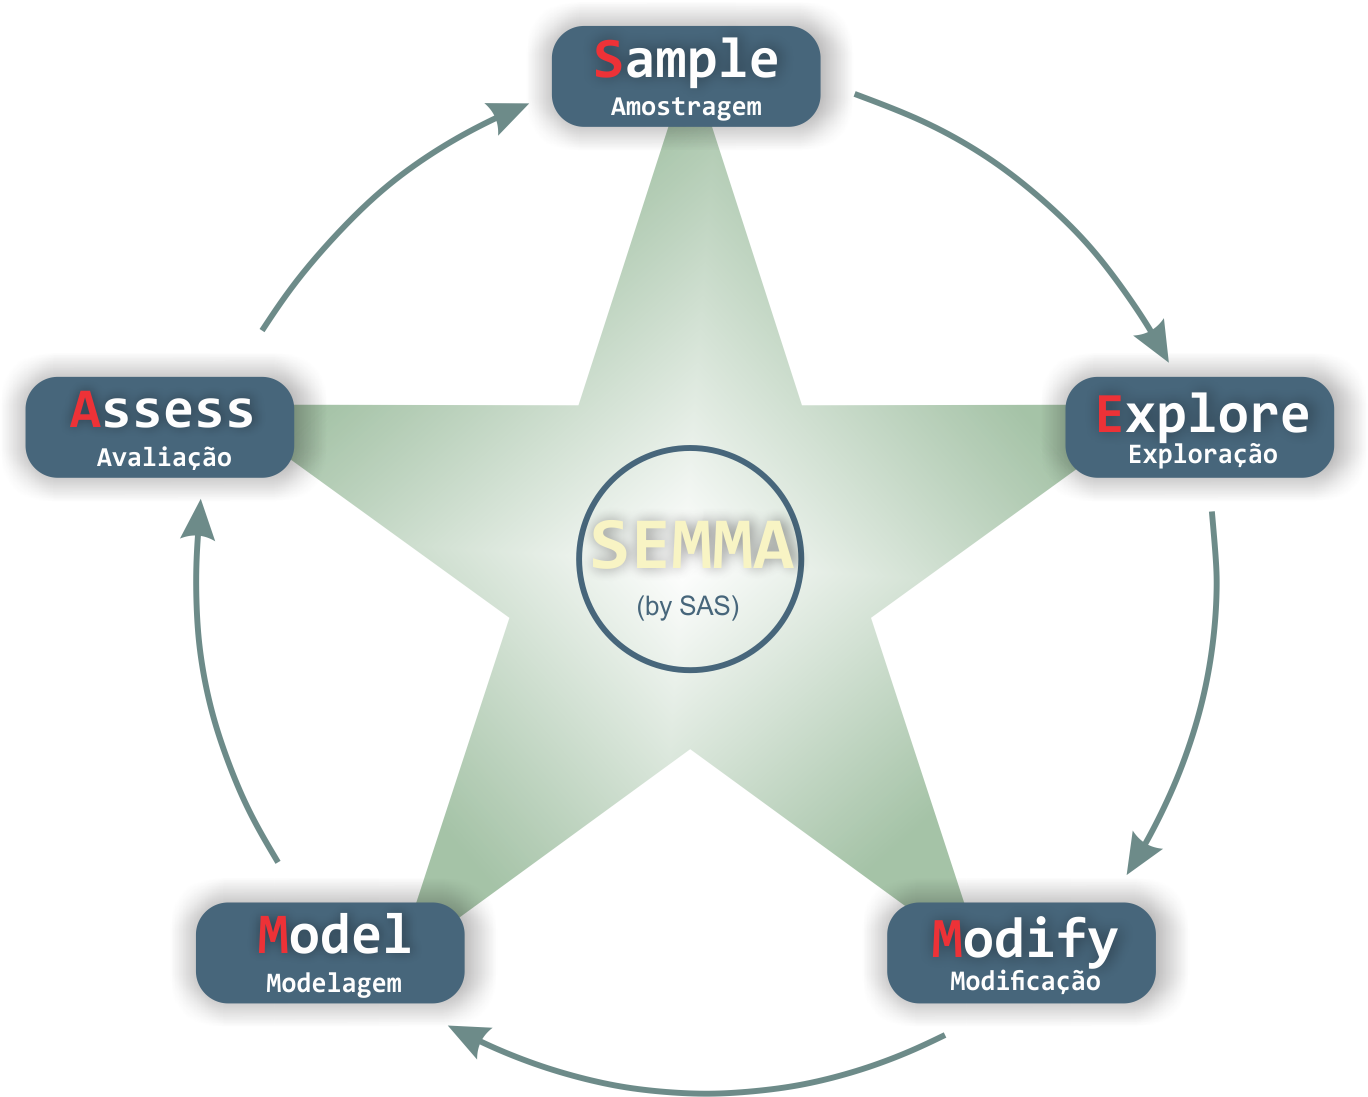
\includegraphics[width=7.29167in,height=\textheight,keepaspectratio]{../../images/semma.png}
\end{center}
\end{frame}

\begin{frame}{SEMMA: Amostragem}
\phantomsection\label{semma-amostragem}
\begin{itemize}
\tightlist
\item
  Nesta fase, o objetivo é selecionar um subconjunto representativo dos
  dados originais.
\end{itemize}

\pause

\begin{itemize}
\tightlist
\item
  É importante garantir que a amostra seja grande o suficiente para
  fornecer resultados precisos e confiáveis.
\end{itemize}
\end{frame}

\begin{frame}{SEMMA: Exploração}
\phantomsection\label{semma-explorauxe7uxe3o}
\begin{itemize}
\tightlist
\item
  Nesta fase, o objetivo é explorar os dados selecionados na etapa
  anterior e identificar padrões ou tendências.
\end{itemize}

\pause

\begin{itemize}
\tightlist
\item
  É importante visualizar os dados para identificar padrões facilmente e
  identificar outliers.
\end{itemize}
\end{frame}

\begin{frame}{SEMMA: Modificação}
\phantomsection\label{semma-modificauxe7uxe3o}
\begin{itemize}
\tightlist
\item
  Nesta fase, o objetivo é transformar os dados de forma apropriada para
  que possam ser usados na modelagem.
\end{itemize}

\pause

\begin{itemize}
\tightlist
\item
  É importante realizar a limpeza dos dados, selecionar as variáveis
  relevantes e transformar os dados para que possam ser usados na
  modelagem.
\end{itemize}
\end{frame}

\begin{frame}{SEMMA: Modelagem}
\phantomsection\label{semma-modelagem}
\begin{itemize}
\tightlist
\item
  Nesta fase, o objetivo é criar e testar modelos usando os dados
  preparados na etapa anterior.
\end{itemize}

\pause

\begin{itemize}
\tightlist
\item
  É importante selecionar as técnicas de modelagem apropriadas e avaliar
  a eficácia do modelo usando conjuntos de dados de treinamento e teste.
\end{itemize}
\end{frame}

\begin{frame}{SEMMA: Avaliação}
\phantomsection\label{semma-avaliauxe7uxe3o}
\begin{itemize}
\tightlist
\item
  Nesta fase, o objetivo é avaliar a eficácia do modelo em relação aos
  critérios de sucesso definidos na fase de amostragem.
\end{itemize}

\pause

\begin{itemize}
\tightlist
\item
  É importante avaliar o modelo em conjuntos de dados de teste
  independentes e garantir que ele atenda aos requisitos do usuário.
\end{itemize}
\end{frame}

\begin{frame}{CRISP-DM}
\phantomsection\label{crisp-dm}
\begin{itemize}
\tightlist
\item
  CRISP-DM (\textbf{CR}oss \textbf{I}ndustry \textbf{S}tandard
  \textbf{P}rocess for \textbf{D}ata \textbf{M}ining) é uma metodologia
  de mineração de dados amplamente utilizada.
\end{itemize}

\pause

\begin{itemize}
\tightlist
\item
  Envolve \textbf{seis etapas}: compreensão do negócio, compreensão dos
  dados, preparação dos dados, modelagem, avaliação e implementação.
\end{itemize}

\pause

\begin{itemize}
\tightlist
\item
  É uma abordagem iterativa e pode ser adaptada para atender a
  necessidades específicas do projeto.
\end{itemize}
\end{frame}

\begin{frame}{CRISP-DM}
\phantomsection\label{crisp-dm-1}
\begin{center}
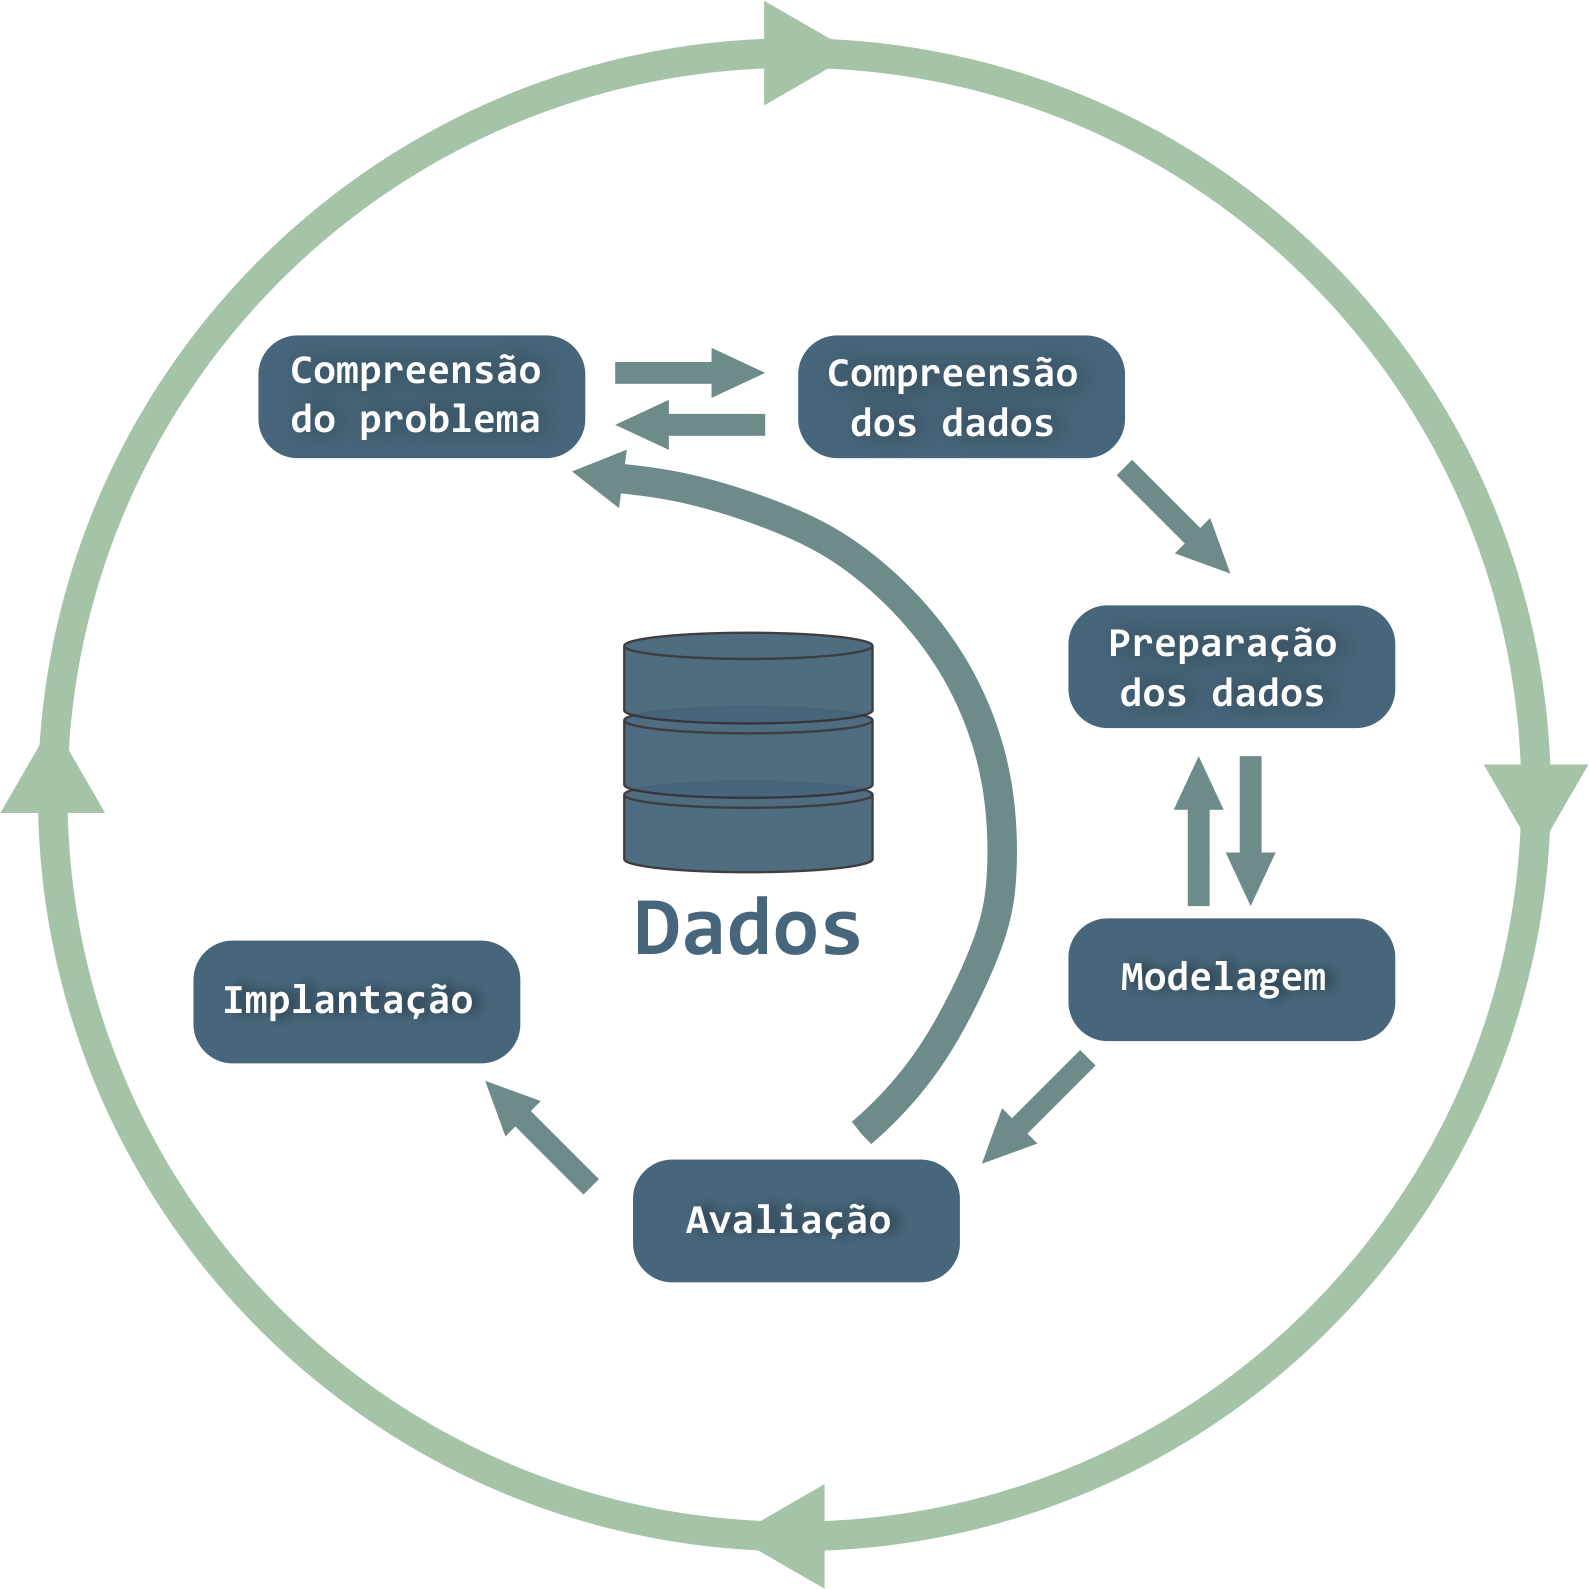
\includegraphics[width=7.29167in,height=\textheight,keepaspectratio]{../../images/crisp.png}
\end{center}
\end{frame}

\begin{frame}{CRISP-DM: Compreensão do negócio}
\phantomsection\label{crisp-dm-compreensuxe3o-do-neguxf3cio}
\begin{itemize}
\tightlist
\item
  Nesta fase, o objetivo é entender os objetivos do projeto, identificar
  as necessidades do usuário e definir os critérios de sucesso.
\end{itemize}

\pause

\begin{itemize}
\tightlist
\item
  É importante definir claramente o escopo do projeto e entender os
  recursos disponíveis.
\end{itemize}
\end{frame}

\begin{frame}{CRISP-DM: Compreensão dos Dados}
\phantomsection\label{crisp-dm-compreensuxe3o-dos-dados}
\begin{itemize}
\tightlist
\item
  Nesta fase, o objetivo é coletar, limpar, integrar e explorar os
  dados.
\end{itemize}

\pause

\begin{itemize}
\tightlist
\item
  É importante identificar a qualidade dos dados, definir as variáveis
  relevantes e compreender a estrutura dos dados.
\end{itemize}
\end{frame}

\begin{frame}{CRISP-DM: Preparação dos Dados}
\phantomsection\label{crisp-dm-preparauxe7uxe3o-dos-dados}
\begin{itemize}
\tightlist
\item
  Nesta fase, o objetivo é selecionar as variáveis relevantes,
  transformar os dados e criar conjuntos de dados de treinamento e
  teste.
\end{itemize}

\pause

\begin{itemize}
\tightlist
\item
  É importante garantir que os dados estejam limpos, completos e
  estruturados de maneira adequada para a modelagem.
\end{itemize}
\end{frame}

\begin{frame}{CRISP-DM: Modelagem}
\phantomsection\label{crisp-dm-modelagem}
\begin{itemize}
\tightlist
\item
  Nesta fase, o objetivo é construir e avaliar modelos que possam prever
  ou classificar novos casos.
\end{itemize}

\pause

\begin{itemize}
\tightlist
\item
  É importante selecionar as técnicas de modelagem apropriadas e avaliar
  a eficácia do modelo usando conjuntos de dados de treinamento e teste.
\end{itemize}
\end{frame}

\begin{frame}{CRISP-DM: Avaliação}
\phantomsection\label{crisp-dm-avaliauxe7uxe3o}
\begin{itemize}
\tightlist
\item
  Nesta fase, o objetivo é avaliar a eficácia do modelo em relação aos
  critérios de sucesso definidos na fase de compreensão do negócio.
\end{itemize}

\pause

\begin{itemize}
\tightlist
\item
  É importante avaliar o modelo em conjuntos de dados de teste
  independentes e garantir que ele atenda aos requisitos do usuário.
\end{itemize}
\end{frame}

\begin{frame}{CRISP-DM: Implantação}
\phantomsection\label{crisp-dm-implantauxe7uxe3o}
\begin{itemize}
\tightlist
\item
  Nesta fase, o objetivo é implantar o modelo em um ambiente de produção
  e monitorá-lo regularmente para garantir que continue a atender aos
  requisitos do usuário.
\end{itemize}

\pause

\begin{itemize}
\tightlist
\item
  É importante desenvolver um plano de implantação e treinamento para
  garantir que o modelo seja adotado pelos usuários.
\end{itemize}
\end{frame}

\begin{frame}{Qual metodologia utilizar?}
\phantomsection\label{qual-metodologia-utilizar}
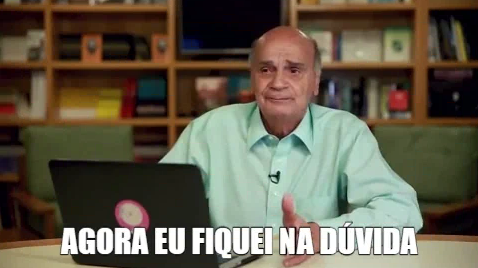
\includegraphics[width=0.7\linewidth,height=\textheight,keepaspectratio]{../../images/drauzio.png}
\end{frame}

\begin{frame}{Qual metodologia utilizar?}
\phantomsection\label{qual-metodologia-utilizar-1}
CRISP-DM, SEMMA e KDD são todas metodologias amplamente utilizadas para
gerenciamento de projetos de mineração de dados.

\pause

CRISP-DM é uma abordagem iterativa em cascata, SEMMA é uma abordagem em
cascata focada no modelo e KDD é uma metodologia mais ampla com três
etapas principais.

\pause

A escolha da metodologia dependerá das necessidades específicas do
projeto e dos recursos disponíveis para o gerenciamento do projeto.
\end{frame}

\begin{frame}{Exemplo aplicado: previsão de churn em telecom}
\phantomsection\label{exemplo-aplicado-previsuxe3o-de-churn-em-telecom}
\textbf{Problema:} prever quais clientes têm maior chance de cancelar o
serviço.

\begin{block}{🔄 O mesmo processo sob diferentes metodologias}
\phantomsection\label{o-mesmo-processo-sob-diferentes-metodologias}
\begin{longtable}[]{@{}llll@{}}
\toprule\noalign{}
\textbf{Etapa} & \textbf{KDD} & \textbf{SEMMA} & \textbf{CRISP-DM} \\
\midrule\noalign{}
\endhead
\textbf{Problema} & --- & --- & Entendimento do Negócio \\
\textbf{Dados} & Seleção & Sample / Explore & Entendimento dos Dados \\
\textbf{Preparação} & Pré-processamento & Modify & Preparação dos
Dados \\
\textbf{Modelo} & Mineração & Model & Modelagem \\
\textbf{Avaliação} & Interpretação & Assess & Avaliação \\
\bottomrule\noalign{}
\end{longtable}
\end{block}
\end{frame}

\begin{frame}
\begin{block}{🧠 O que estamos vendo?}
\phantomsection\label{o-que-estamos-vendo}
\begin{itemize}
\tightlist
\item
  As três metodologias seguem o mesmo fluxo:

  \begin{itemize}
  \tightlist
  \item
    problema → dados → preparação → modelo → avaliação
  \end{itemize}
\end{itemize}
\end{block}

\begin{block}{🔍 Diferenças principais}
\phantomsection\label{diferenuxe7as-principais}
\begin{itemize}
\tightlist
\item
  \textbf{KDD} → foco em descoberta de conhecimento\\
\item
  \textbf{SEMMA} → foco na modelagem\\
\item
  \textbf{CRISP-DM} → foco no problema de negócio
\end{itemize}

\begin{tcolorbox}[enhanced jigsaw, toprule=.15mm, breakable, colframe=quarto-callout-important-color-frame, left=2mm, bottomrule=.15mm, leftrule=.75mm, arc=.35mm, rightrule=.15mm, colback=white, opacityback=0]
\begin{minipage}[t]{5.5mm}
\textcolor{quarto-callout-important-color}{\faExclamation}
\end{minipage}%
\begin{minipage}[t]{\textwidth - 5.5mm}

\textbf{Mensagem principal:}\\
Mineração de dados não é só modelar: é um processo completo.

\end{minipage}%
\end{tcolorbox}
\end{block}
\end{frame}

\begin{frame}{Tarefas e técnicas de mineração de dados}
\phantomsection\label{tarefas-e-tuxe9cnicas-de-minerauxe7uxe3o-de-dados}
Uma \textbf{tarefa} de mineração de dados determina o \textbf{tipo de
problema} que será resolvido pelo processo de mineração de dados.

\begin{itemize}
\tightlist
\item
  Podem ser \textbf{descritivas} ou \textbf{preditivas}.
\end{itemize}

\pause

Já a \textbf{técnica}, representa o \textbf{algoritmo} que pode ser
empregado para a \textbf{execução da tarefa}.
\end{frame}

\begin{frame}{Tarefas e técnicas de mineração de dados}
\phantomsection\label{tarefas-e-tuxe9cnicas-de-minerauxe7uxe3o-de-dados-1}
As \textbf{tarefas de mineração de dados} incluem: classificação,
clustering, regressão, associação e detecção de anomalias.

\pause

Cada uma dessas tarefas tem um objetivo específico na análise de dados.
\end{frame}

\begin{frame}{Classificação}
\phantomsection\label{classificauxe7uxe3o}
\begin{columns}[T]
\begin{column}{0.5\linewidth}
\begin{center}
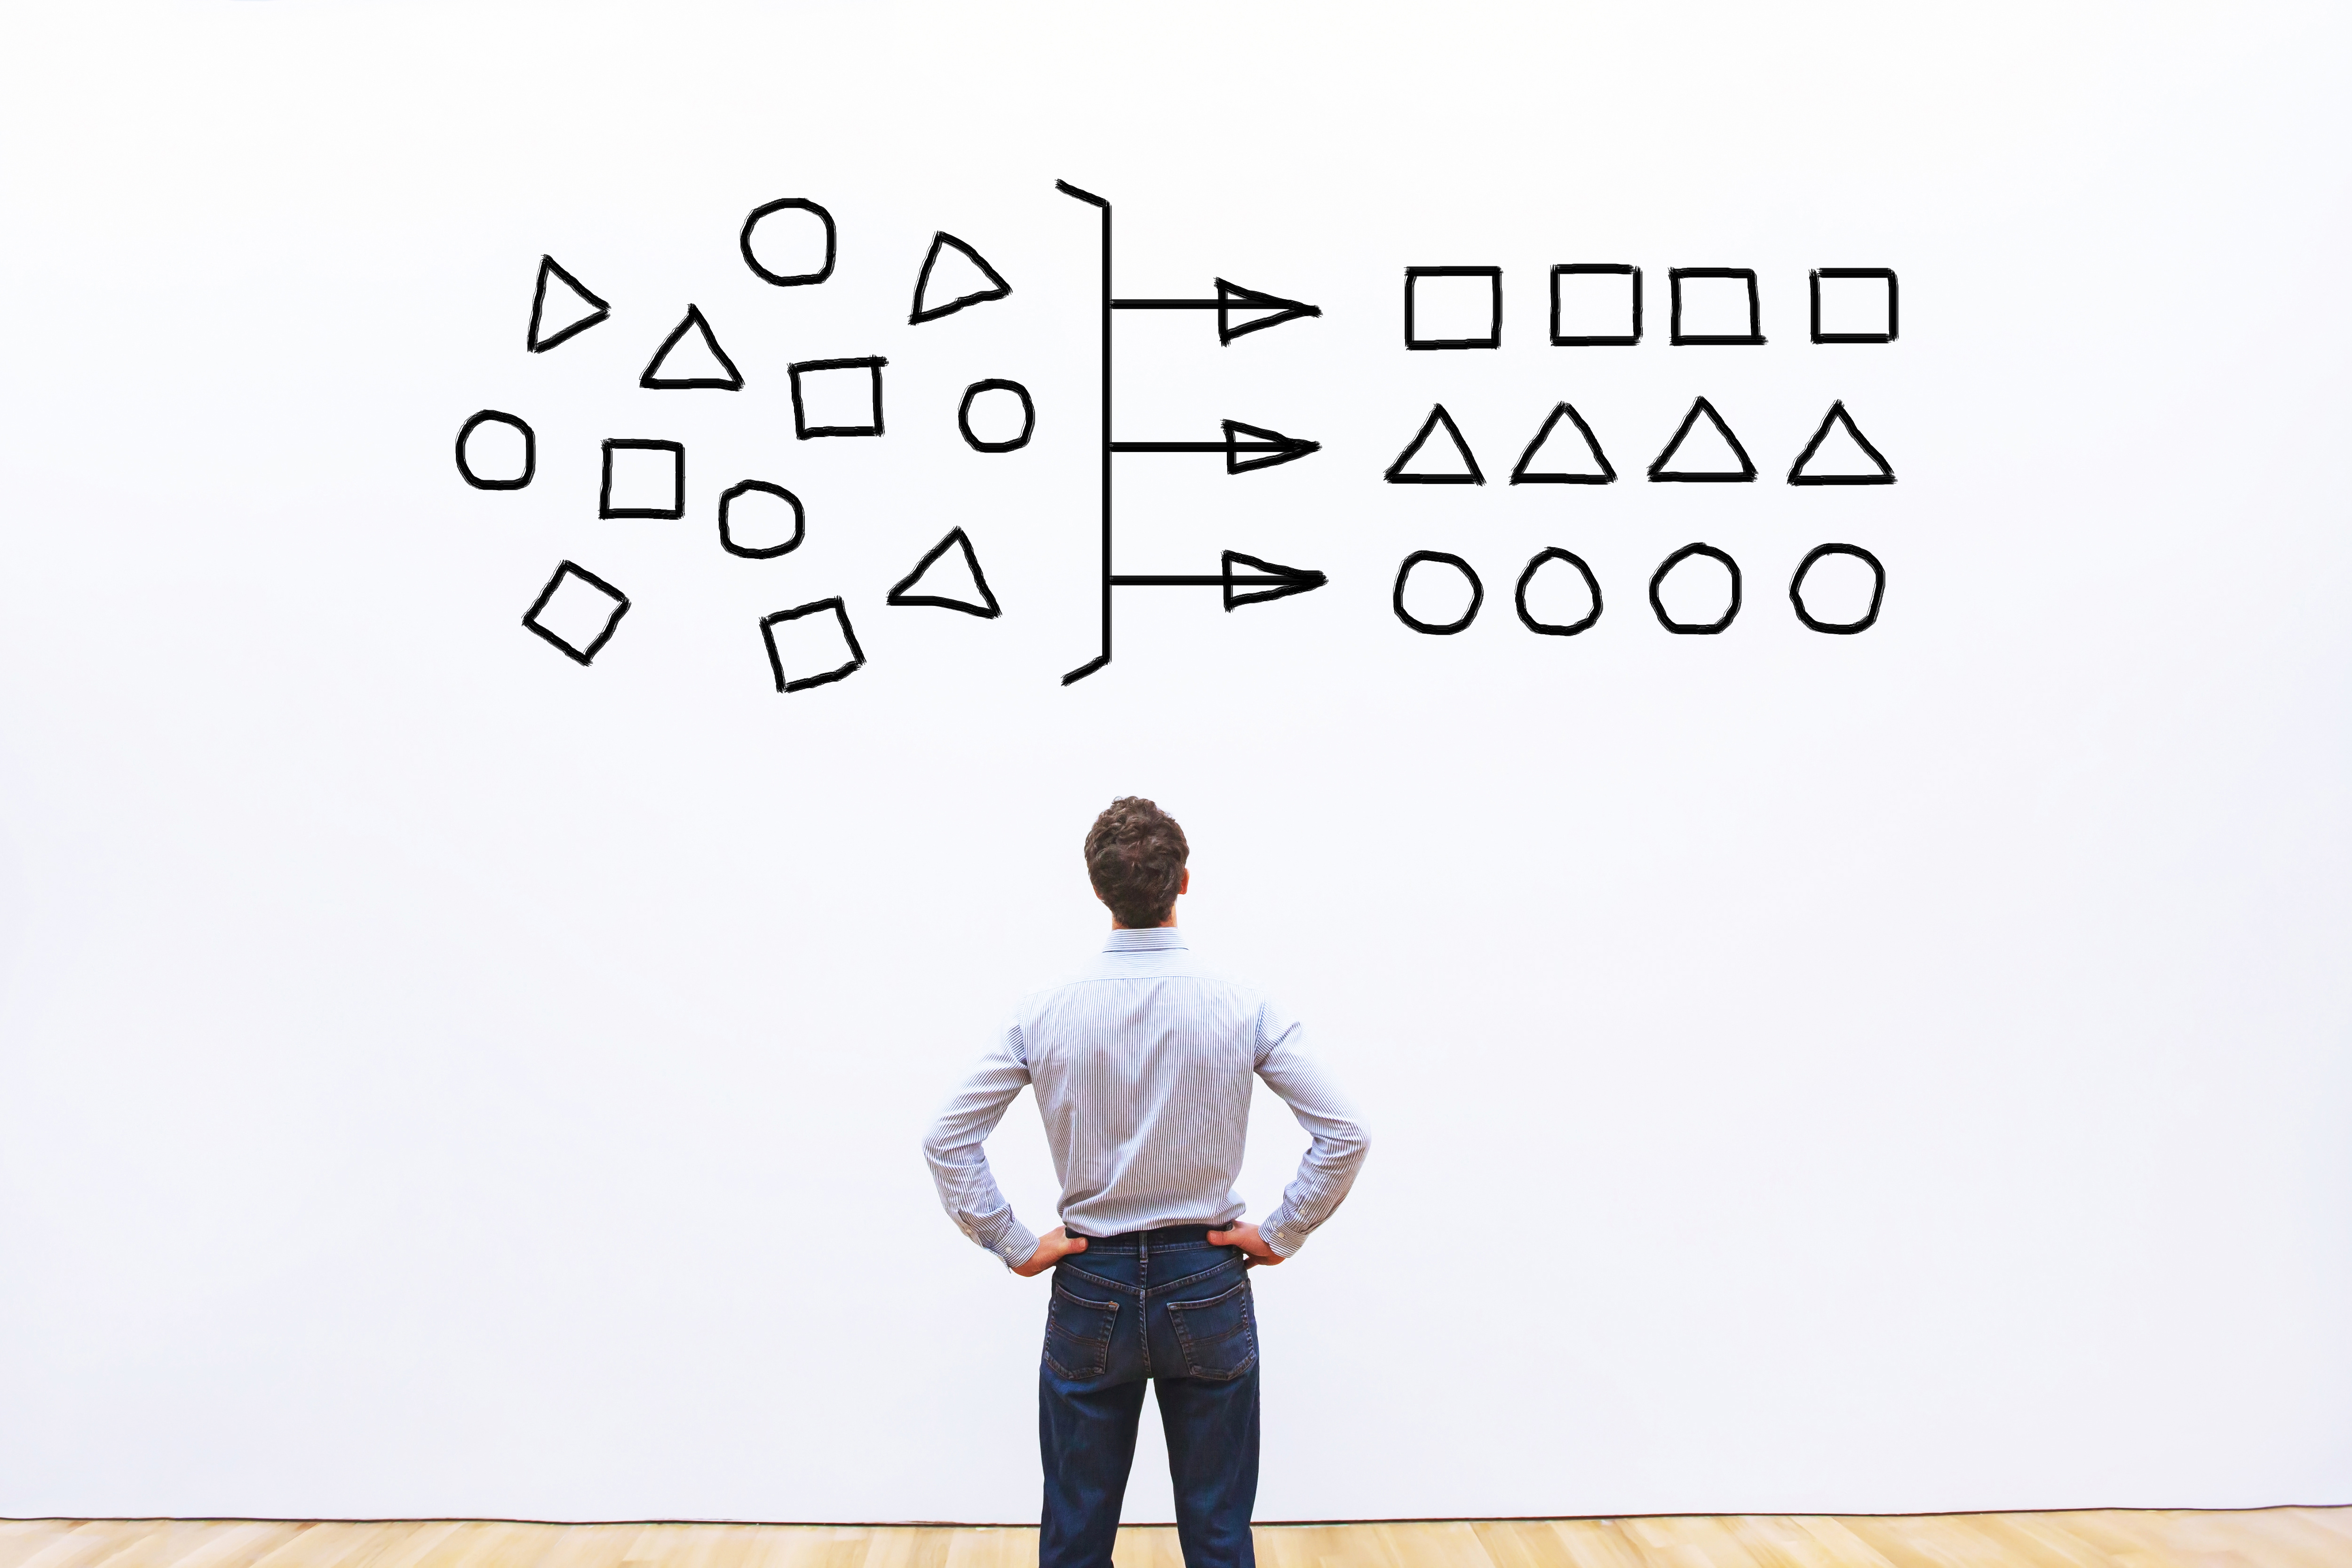
\includegraphics[width=8.33333in,height=\textheight,keepaspectratio]{../../images/classificacao.jpeg}
\end{center}
\end{column}

\begin{column}{0.5\linewidth}
\end{column}
\end{columns}
\end{frame}

\begin{frame}{Clusterização}
\phantomsection\label{clusterizauxe7uxe3o}
\begin{columns}[T]
\begin{column}{0.5\linewidth}
\end{column}

\begin{column}{0.5\linewidth}
\begin{center}
\includegraphics[width=8.33333in,height=\textheight,keepaspectratio]{../../images/cluster.jpeg}
\end{center}
\end{column}
\end{columns}
\end{frame}

\begin{frame}{Regressão ou predição}
\phantomsection\label{regressuxe3o-ou-prediuxe7uxe3o}
\begin{columns}[T]
\begin{column}{0.5\linewidth}
\end{column}

\begin{column}{0.5\linewidth}
\begin{center}
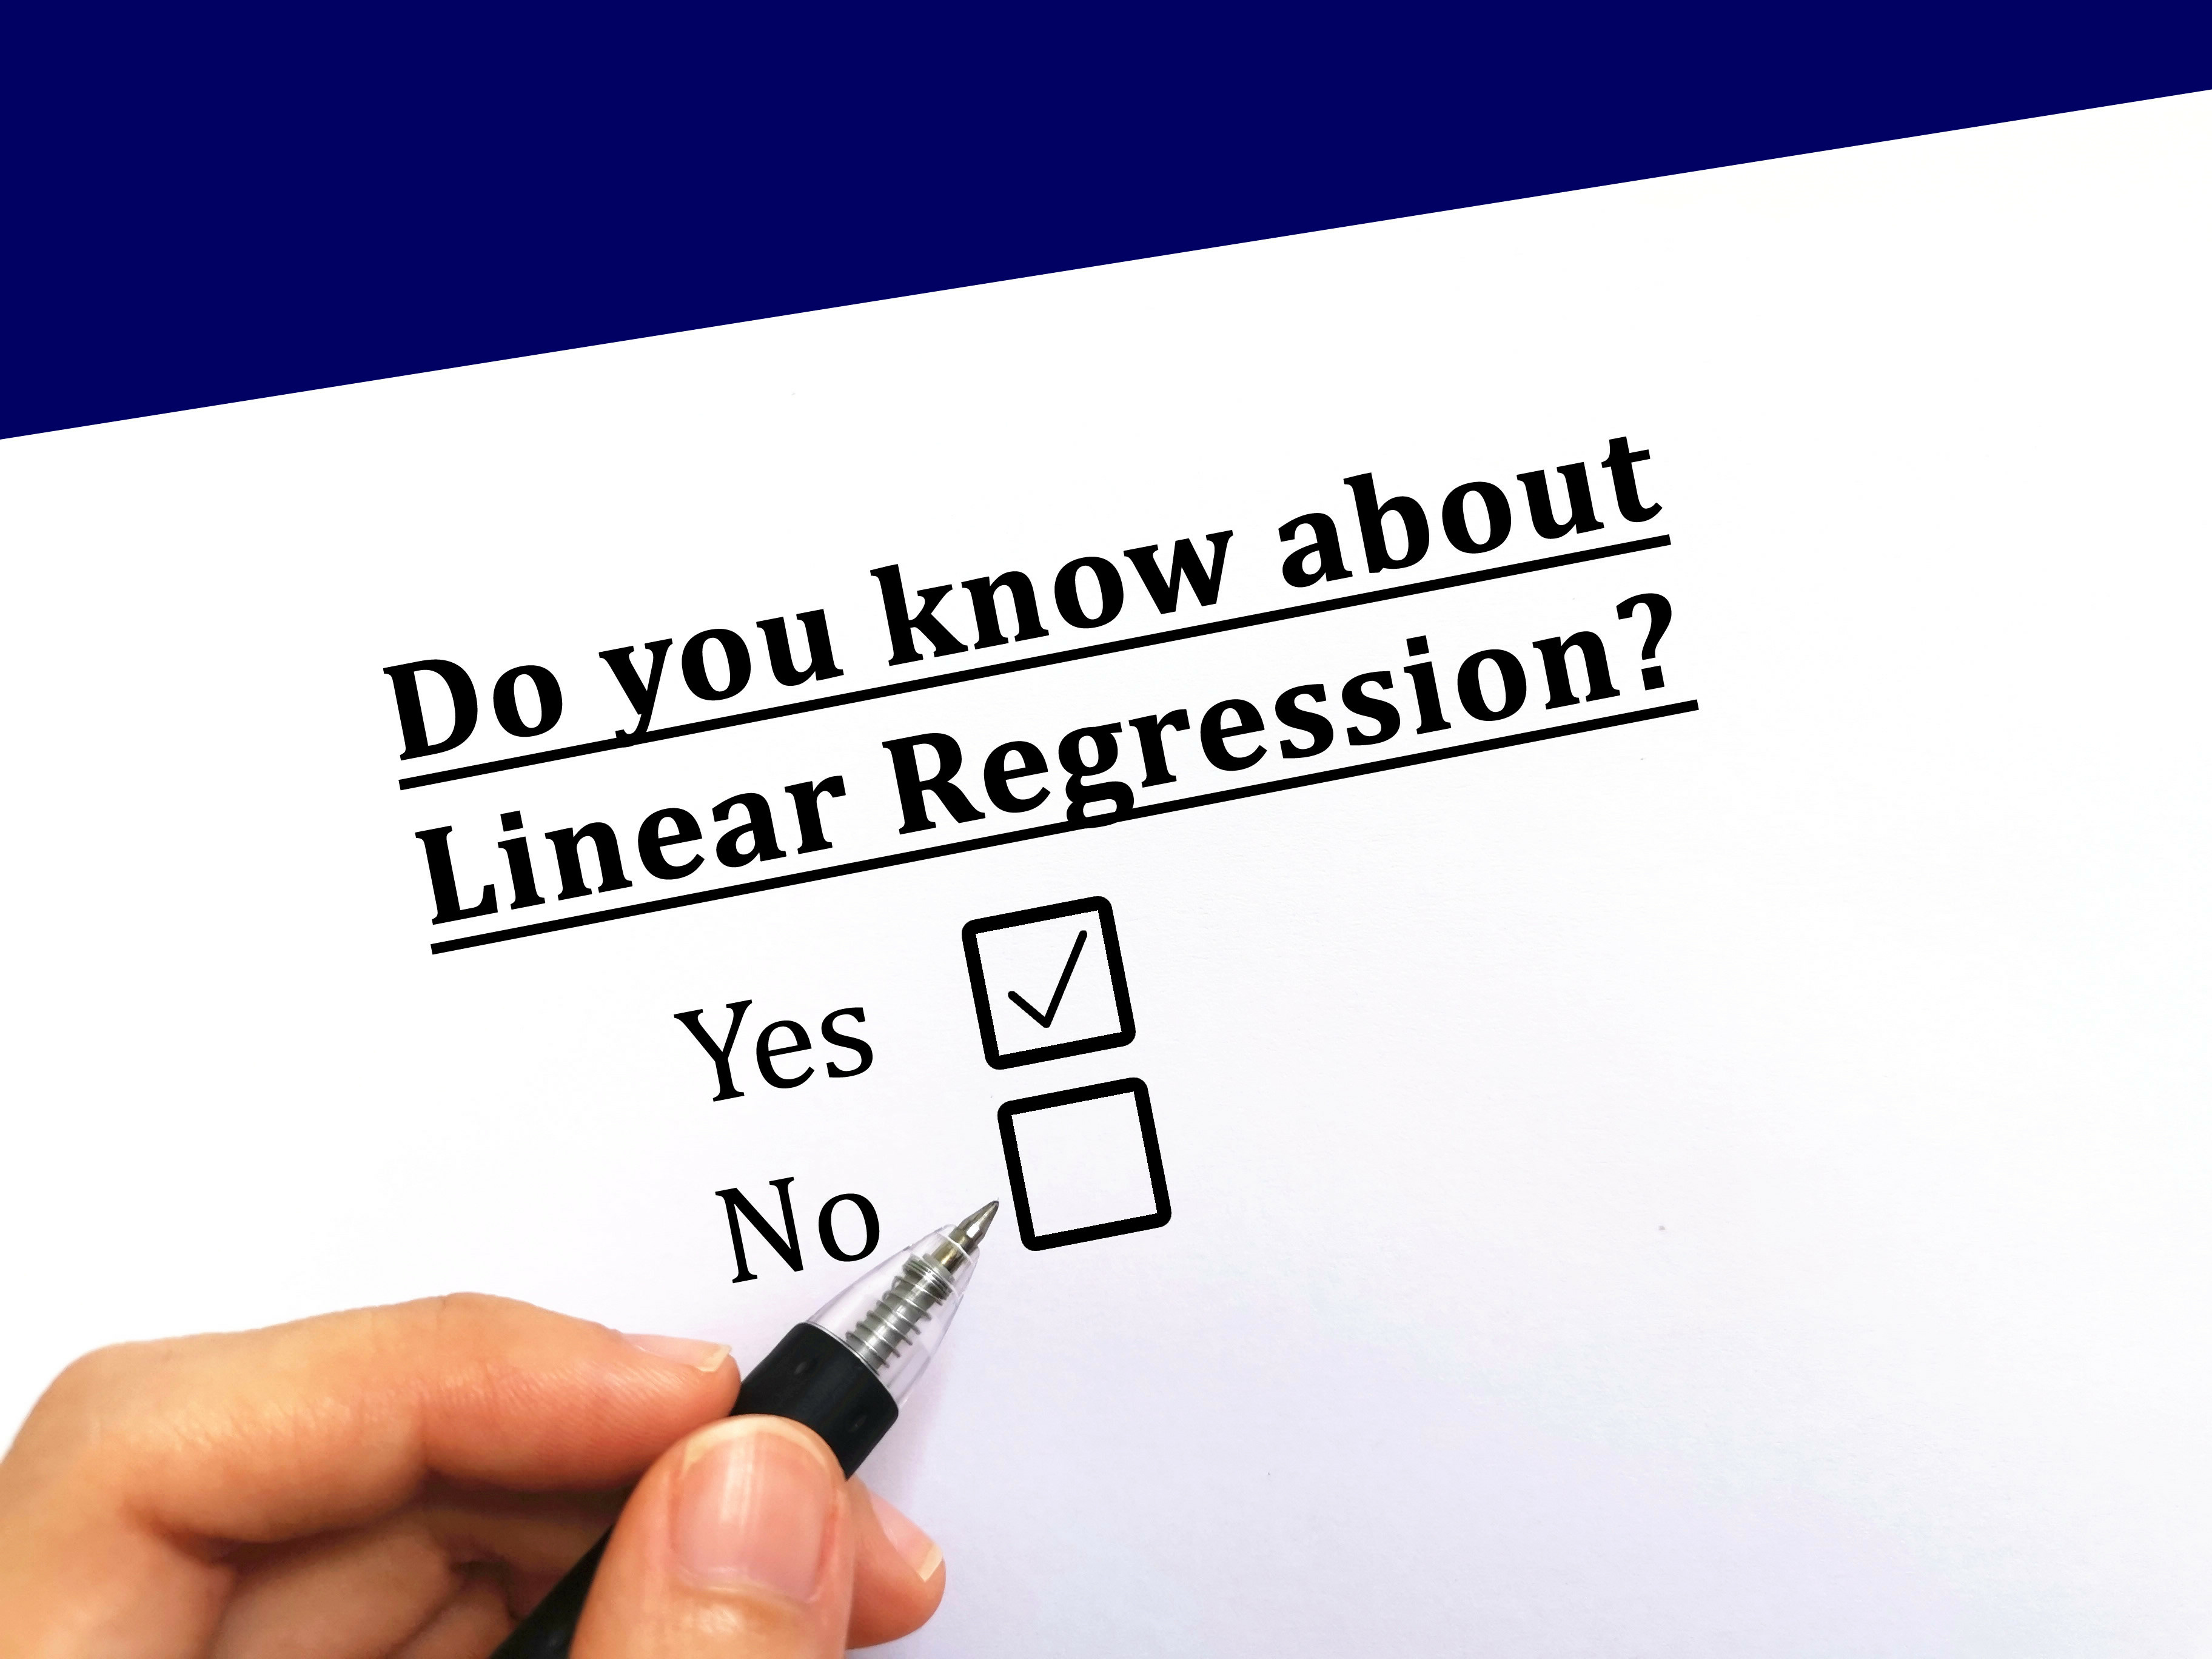
\includegraphics[width=8.33333in,height=\textheight,keepaspectratio]{../../images/regressao.jpeg}
\end{center}
\end{column}
\end{columns}

As técnicas de regressão incluem: regressão linear, regressão logística,
etc.
\end{frame}

\begin{frame}{Associação}
\phantomsection\label{associauxe7uxe3o}
\begin{columns}[T]
\begin{column}{0.5\linewidth}
\begin{center}
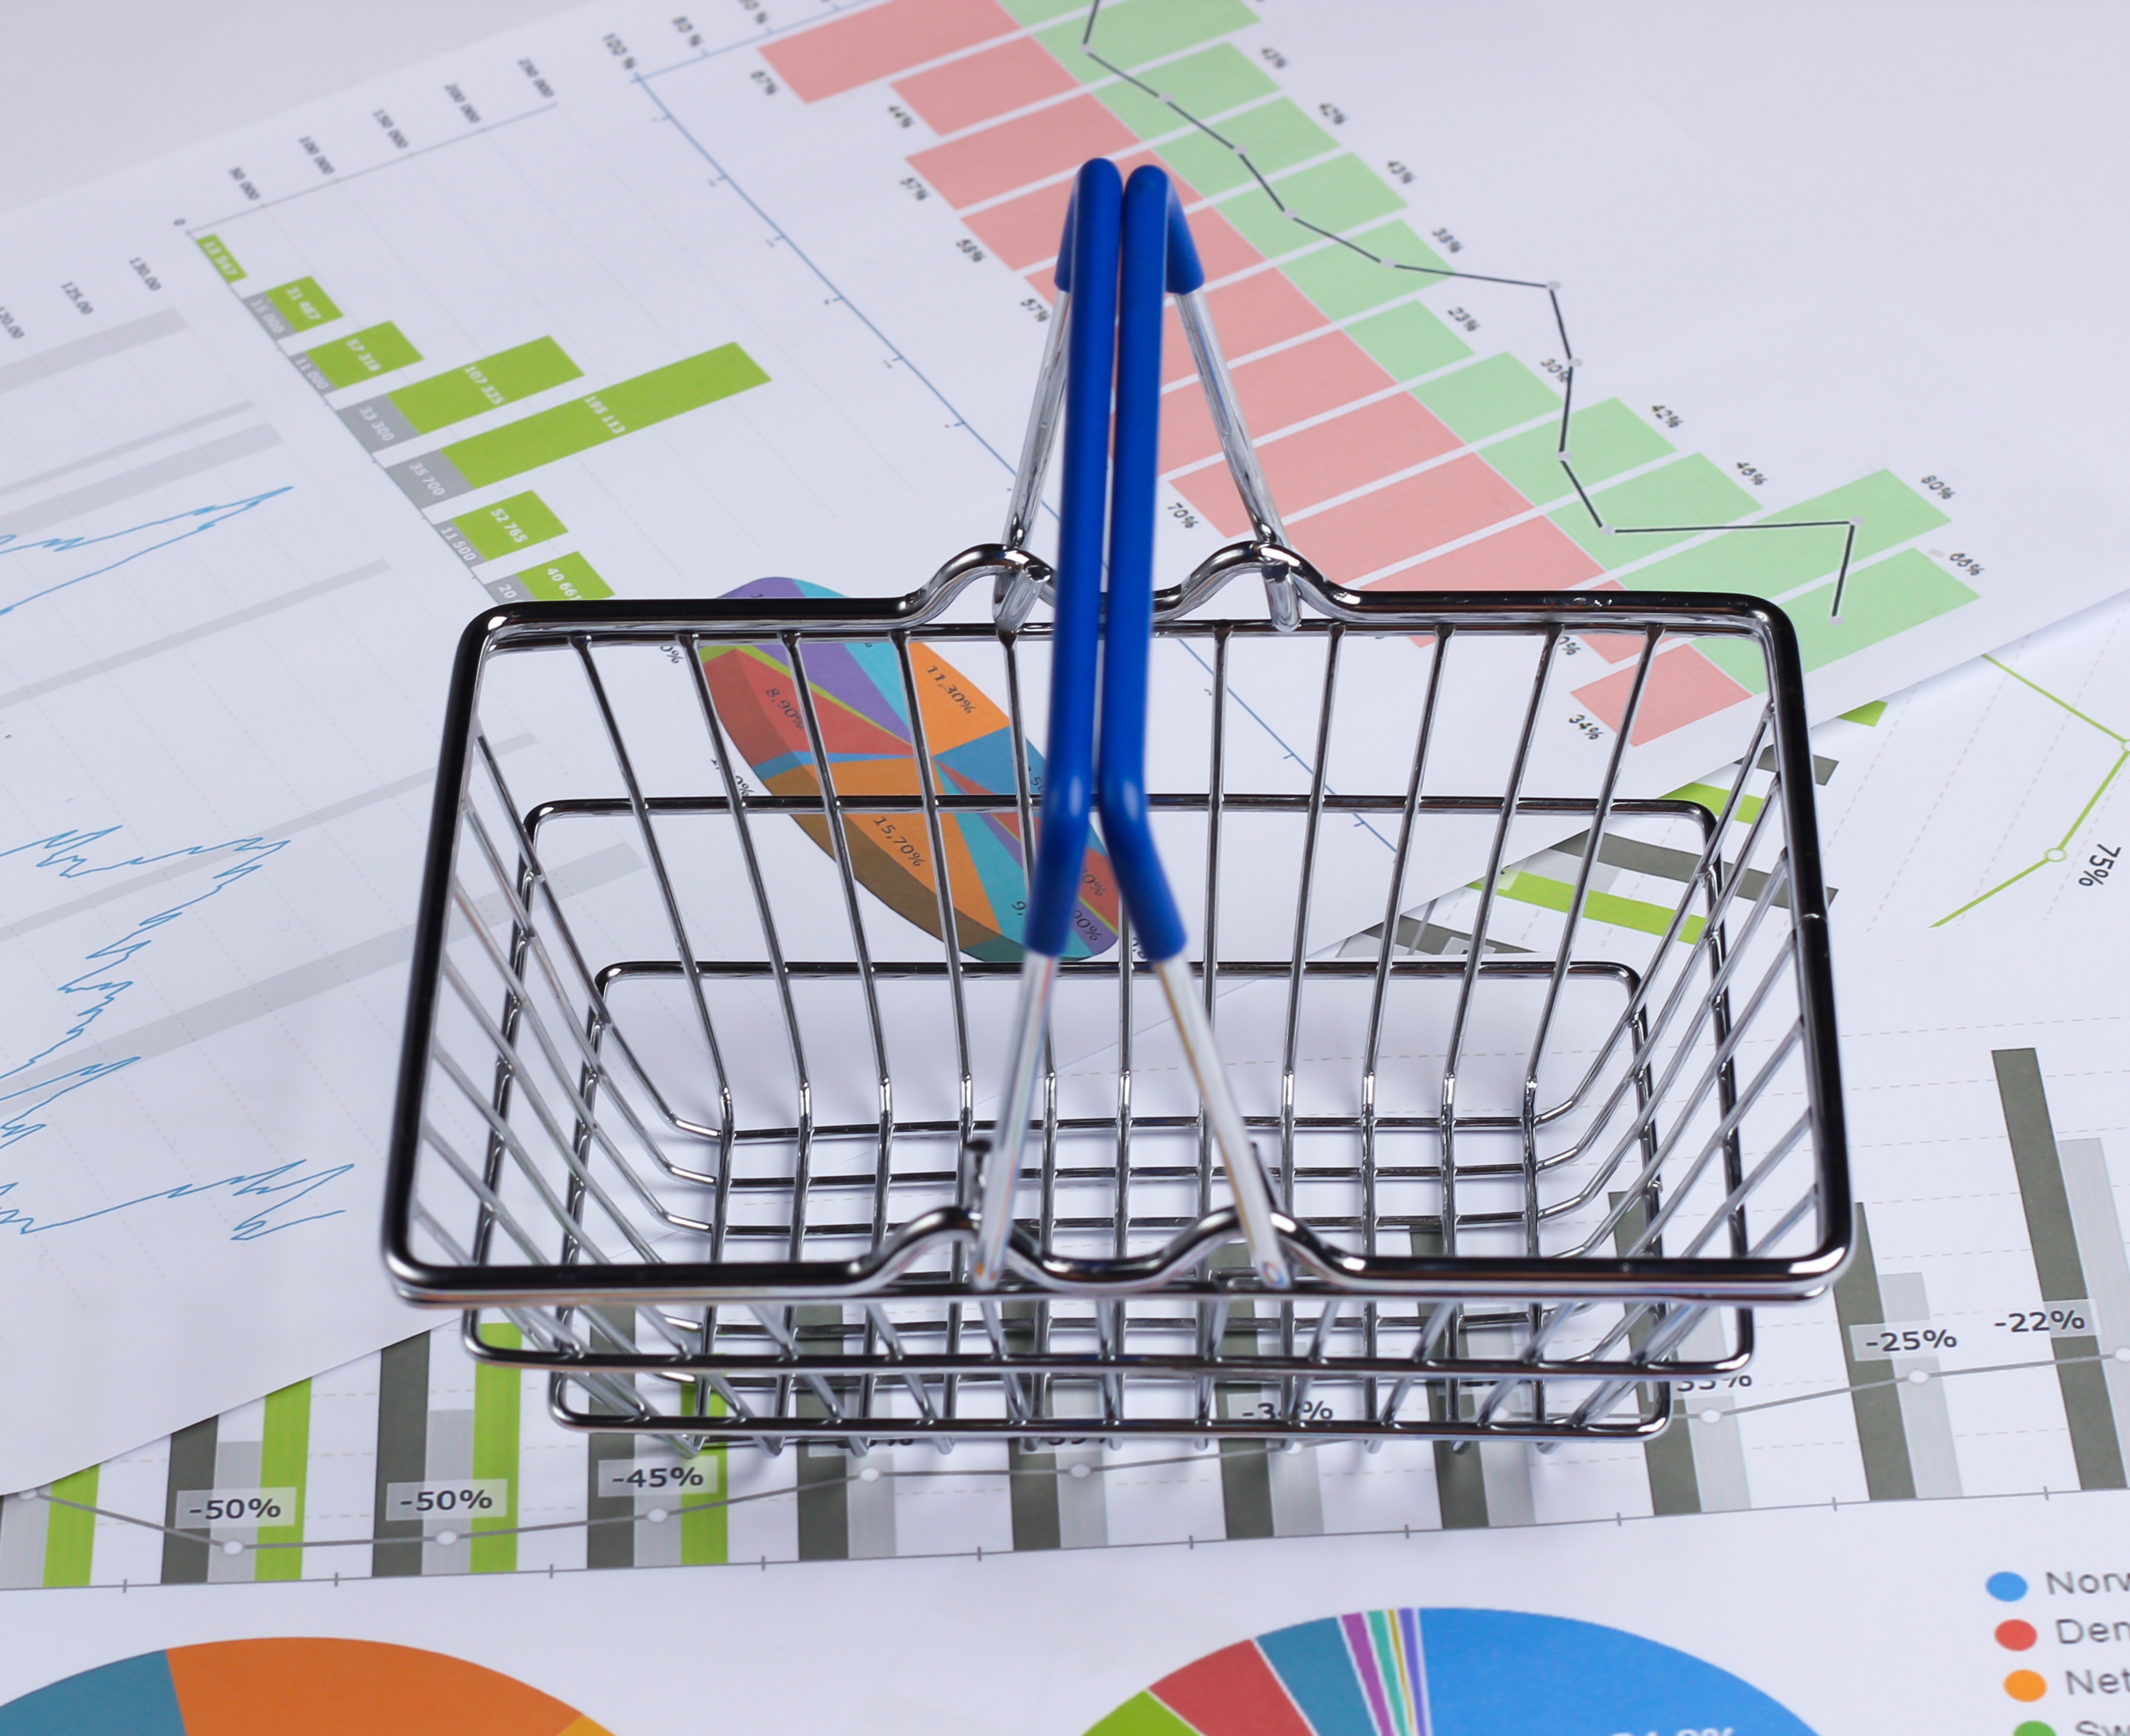
\includegraphics[width=8.33333in,height=\textheight,keepaspectratio]{../../images/associacao.jpeg}
\end{center}
\end{column}

\begin{column}{0.5\linewidth}
\end{column}
\end{columns}
\end{frame}

\begin{frame}{Detecção de anomalias}
\phantomsection\label{detecuxe7uxe3o-de-anomalias}
\begin{columns}[T]
\begin{column}{0.5\linewidth}
\end{column}

\begin{column}{0.5\linewidth}
\begin{center}

\includegraphics[width=8.33333in,height=\textheight,keepaspectratio]{../../images/anomalia.jpeg}
\end{center}
\end{column}
\end{columns}
\end{frame}

\begin{frame}{Importância da definição dos objetivos}
\phantomsection\label{importuxe2ncia-da-definiuxe7uxe3o-dos-objetivos}
Enquanto isso, no
\href{https://pt.wikipedia.org/wiki/Alice_no_País_das_Maravilhas}{país
das maravilhas}\ldots{}

\begin{center}
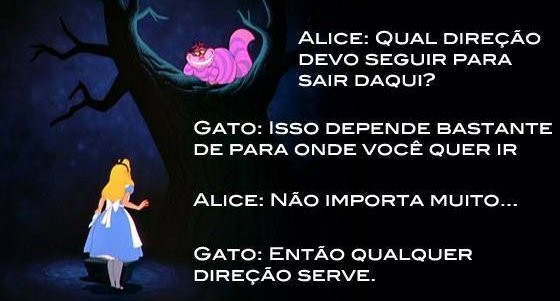
\includegraphics[width=6.25in,height=\textheight,keepaspectratio]{../../images/alice.jpeg}
\end{center}
\end{frame}

\begin{frame}{Definição dos objetivos}
\phantomsection\label{definiuxe7uxe3o-dos-objetivos}
Definir \textbf{claramente os objetivos da análise} de dados é
\textbf{fundamental para o sucesso} do projeto.

\pause

Os objetivos devem ser \textbf{específicos}, \textbf{mensuráveis},
\textbf{alcançáveis}, \textbf{relevantes} e ter um \textbf{prazo
estabelecido}
(\href{https://deolhonofuturo.uninter.com/metodologia-smart/?gclid=CjwKCAjw8-OhBhB5EiwADyoY1TeU-iDp_vyUvve_TLMgNiTOO2t_ZZKzN3bCyLVwzB52-c6NrwJLBhoC3tEQAvD_BwE}{SMART}).

\pause

\begin{itemize}
\item
  Por exemplo, suponha que uma empresa queira aumentar as vendas em uma
  determinada região.

  \begin{itemize}
  \tightlist
  \item
    Usando a metodologia SMART, a empresa pode definir o objetivo da
    seguinte maneira:
  \end{itemize}
\end{itemize}
\end{frame}

\begin{frame}{Definição dos objetivos}
\phantomsection\label{definiuxe7uxe3o-dos-objetivos-1}
\begin{itemize}
\item
  \textbf{Específico:} O objetivo deve ser específico e detalhado.

  \begin{itemize}
  \tightlist
  \item
    Por exemplo, ``Aumentar as vendas de determinada categoria de
    produtos na região em 10\% no próximo trimestre''.
  \end{itemize}
\end{itemize}

\pause

\begin{itemize}
\item
  \textbf{Mensurável:} O objetivo deve ser mensurável para que possa ser
  avaliado.

  \begin{itemize}
  \tightlist
  \item
    Por exemplo, a empresa pode usar dados de vendas para medir o
    progresso em relação à meta.
  \end{itemize}
\end{itemize}

\pause

\begin{itemize}
\item
  \textbf{Alcançável:} O objetivo deve ser alcançável para evitar
  frustração e desânimo da equipe.

  \begin{itemize}
  \tightlist
  \item
    A empresa pode avaliar a capacidade da equipe, recursos disponíveis
    e condições de mercado para determinar se a meta é alcançável.
  \end{itemize}
\end{itemize}
\end{frame}

\begin{frame}{Definição dos objetivos}
\phantomsection\label{definiuxe7uxe3o-dos-objetivos-2}
\begin{itemize}
\item
  \textbf{Relevante:} O objetivo deve ser relevante para os objetivos de
  negócios da empresa.

  \begin{itemize}
  \tightlist
  \item
    A meta de aumentar as vendas em uma determinada região deve estar
    alinhada com os objetivos de negócios da empresa.
  \end{itemize}
\end{itemize}

\pause

\begin{itemize}
\item
  \textbf{Temporal:} O objetivo deve ser definido em um prazo
  determinado.

  \begin{itemize}
  \tightlist
  \item
    Por exemplo, a meta deve ser alcançada em três meses.
  \end{itemize}
\end{itemize}
\end{frame}

\begin{frame}{Definição dos objetivos}
\phantomsection\label{definiuxe7uxe3o-dos-objetivos-3}
Com a definição \textbf{clara} do objetivo usando a \textbf{metodologia
SMART}, a empresa pode traçar um \textbf{plano de ação}, coletar dados
relevantes, realizar análises para identificar as causas da queda nas
vendas, e implementar medidas para atingir a meta.

\pause

A empresa também pode monitorar o progresso e ajustar as medidas se
necessário para garantir que a meta seja alcançada no prazo
estabelecido.
\end{frame}

\begin{frame}{Importância de entender o problema}
\phantomsection\label{importuxe2ncia-de-entender-o-problema}
\begin{center}

\includegraphics[width=0.6\linewidth,height=\textheight,keepaspectratio]{../../images/problem.png}
\end{center}
\end{frame}

\begin{frame}{Importância de entender o problema}
\phantomsection\label{importuxe2ncia-de-entender-o-problema-1}
\begin{center}
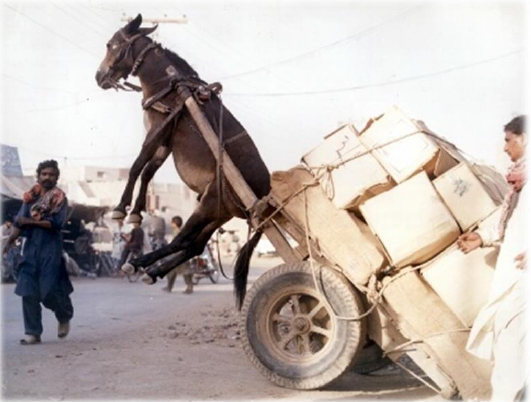
\includegraphics[width=6.25in,height=\textheight,keepaspectratio]{../../images/fig_01.png}
\end{center}
\end{frame}

\begin{frame}{Importância de entender o problema}
\phantomsection\label{importuxe2ncia-de-entender-o-problema-2}
\begin{center}
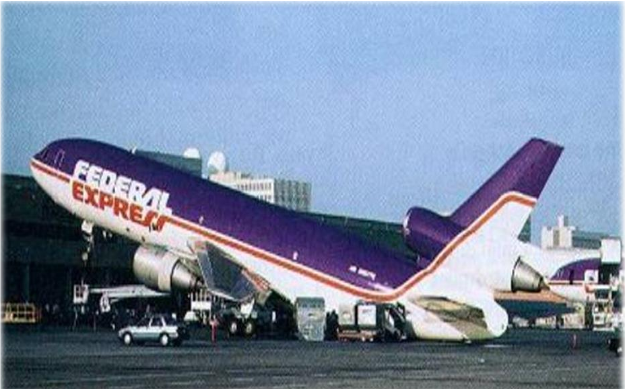
\includegraphics[width=6.25in,height=\textheight,keepaspectratio]{../../images/fig_02.png}
\end{center}
\end{frame}

\begin{frame}{Importância de entender o problema}
\phantomsection\label{importuxe2ncia-de-entender-o-problema-3}
\begin{center}
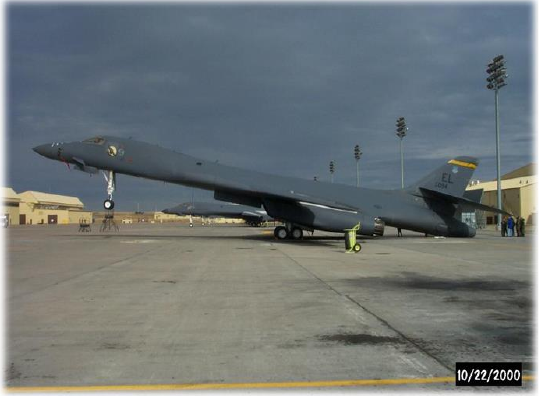
\includegraphics[width=6.25in,height=\textheight,keepaspectratio]{../../images/fig_03.png}
\end{center}
\end{frame}

\begin{frame}{Técnica dos cinco porquês}
\phantomsection\label{tuxe9cnica-dos-cinco-porquuxeas}
\begin{columns}[T]
\begin{column}{0.5\linewidth}
\begin{center}
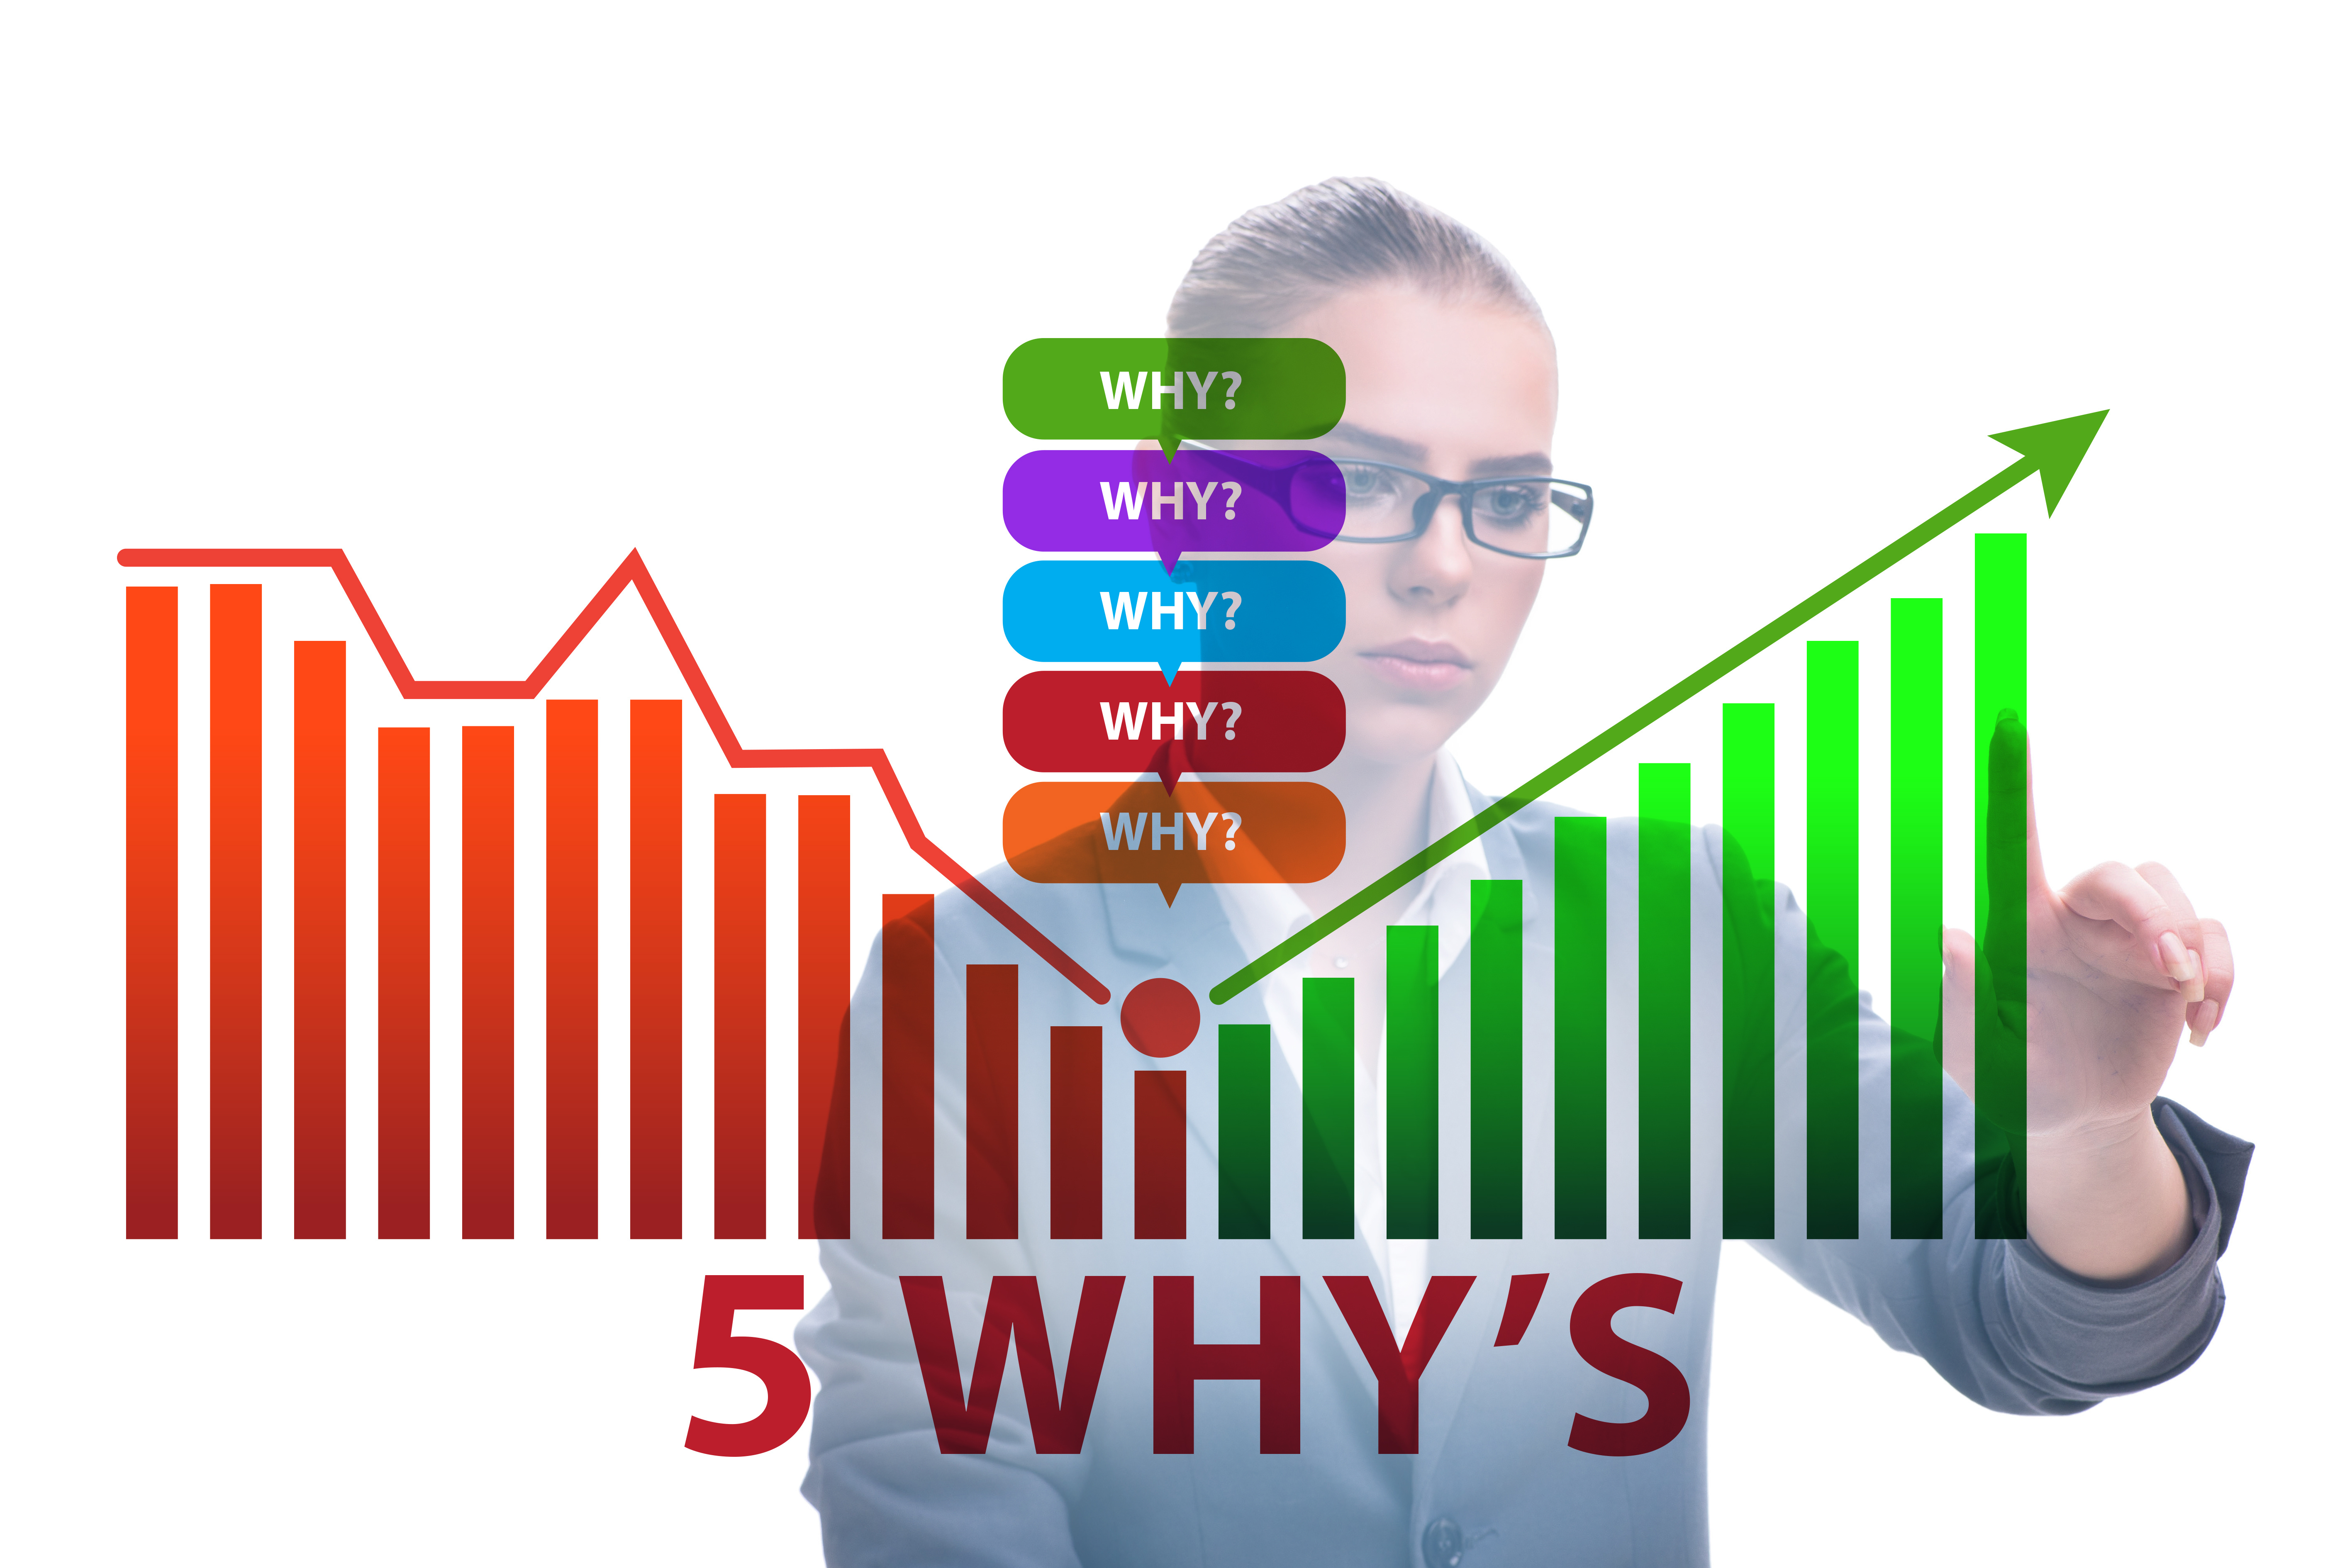
\includegraphics[width=8.33333in,height=\textheight,keepaspectratio]{../../images/5pq.jpeg}
\end{center}
\end{column}

\begin{column}{0.5\linewidth}
\end{column}
\end{columns}
\end{frame}

\begin{frame}{Técnica dos cinco porquês}
\phantomsection\label{tuxe9cnica-dos-cinco-porquuxeas-1}
O processo da técnica dos cinco porquês pode ser resumido nas seguintes
etapas:

\pause

\begin{enumerate}
\tightlist
\item
  \textbf{Identificar o problema:} Comece identificando o problema que
  precisa ser resolvido.
\end{enumerate}

\pause

\begin{enumerate}
\setcounter{enumi}{1}
\tightlist
\item
  \textbf{Fazer a primeira pergunta:} Pergunte ``Por que o problema
  ocorreu?'' e identifique a causa mais provável.
\end{enumerate}

\pause

\begin{enumerate}
\setcounter{enumi}{2}
\tightlist
\item
  \textbf{Fazer a segunda pergunta:} Pergunte ``Por que a causa
  identificada na pergunta anterior ocorreu?'' e identifique a causa
  mais provável.
\end{enumerate}
\end{frame}

\begin{frame}{Técnica dos cinco porquês}
\phantomsection\label{tuxe9cnica-dos-cinco-porquuxeas-2}
\begin{enumerate}
\setcounter{enumi}{3}
\tightlist
\item
  \textbf{Continuar com as perguntas subsequentes:} Continue fazendo
  perguntas sucessivas até que a causa raiz seja identificada.
\end{enumerate}

\pause

\begin{enumerate}
\setcounter{enumi}{4}
\tightlist
\item
  \textbf{Resolver o problema:} Uma vez que a causa raiz é identificada,
  é possível implementar soluções para resolver o problema.
\end{enumerate}

\pause

{👉} É importante notar que, embora a técnica dos cinco porquês seja uma
técnica útil, ela não é uma solução universal para todos os problemas.

\begin{itemize}
\tightlist
\item
  Às vezes, a causa raiz de um problema pode ser mais complexa e exigir
  técnicas de análise mais avançadas.
\item
  Além disso, é importante não se limitar a apenas cinco perguntas se
  necessário para chegar à causa raiz do problema.
\end{itemize}
\end{frame}

\begin{frame}{Exemplo do uso da técnica dos cinco porquês}
\phantomsection\label{exemplo-do-uso-da-tuxe9cnica-dos-cinco-porquuxeas}
\pause

\begin{enumerate}
\tightlist
\item
  Por que o faturamento da empresa diminuiu no último trimestre?
\end{enumerate}

\begin{itemize}
\tightlist
\item
  \textbf{Resposta:} Porque as vendas de um dos produtos mais vendidos
  caíram.
\end{itemize}

\pause

\begin{enumerate}
\setcounter{enumi}{1}
\tightlist
\item
  Por que as vendas do produto mais vendido caíram?
\end{enumerate}

\begin{itemize}
\tightlist
\item
  \textbf{Resposta:} Porque a concorrência começou a oferecer preços
  mais baixos.
\end{itemize}

\pause

\begin{enumerate}
\setcounter{enumi}{2}
\tightlist
\item
  Por que a concorrência começou a oferecer preços mais baixos?
\end{enumerate}

\begin{itemize}
\tightlist
\item
  \textbf{Resposta:} Porque um novo concorrente entrou no mercado e
  começou a oferecer preços mais baixos para ganhar participação de
  mercado.
\end{itemize}
\end{frame}

\begin{frame}{Exemplo do uso da técnica dos cinco porquês}
\phantomsection\label{exemplo-do-uso-da-tuxe9cnica-dos-cinco-porquuxeas-1}
\begin{enumerate}
\setcounter{enumi}{3}
\tightlist
\item
  Por que o novo concorrente conseguiu oferecer preços mais baixos?
\end{enumerate}

\begin{itemize}
\tightlist
\item
  \textbf{Resposta:} Porque ele tem custos de produção mais baixos do
  que a nossa empresa.
\end{itemize}

\pause

\begin{enumerate}
\setcounter{enumi}{4}
\tightlist
\item
  Por que nossos custos de produção são mais altos do que os do novo
  concorrente?
\end{enumerate}

\begin{itemize}
\tightlist
\item
  \textbf{Resposta:} Porque não atualizamos nossos equipamentos de
  produção há anos, o que torna nosso processo menos eficiente e mais
  caro.
\end{itemize}
\end{frame}

\begin{frame}{Exemplo do uso da técnica dos cinco porquês}
\phantomsection\label{exemplo-do-uso-da-tuxe9cnica-dos-cinco-porquuxeas-2}
👉 Com essa análise, a causa raiz do problema do faturamento da empresa
ter diminuído no último trimestre foi identificada: \textbf{a falta de
atualização dos equipamentos de produção}.

\pause

\begin{itemize}
\tightlist
\item
  De posse dessa informação, a empresa pode agora tomar medidas para
  atualizar seus equipamentos de produção e aumentar sua eficiência para
  voltar a ter um faturamento maior.
\end{itemize}
\end{frame}

\begin{frame}{References}
\phantomsection\label{references}
\phantomsection\label{refs}
\begin{CSLReferences}{1}{0}
\bibitem[\citeproctext]{ref-naisbitt1982megatrends}
Naisbitt, J. 1982. \emph{Megatrends: Ten New Directions Transforming Our
Lives}. Megatrends: Ten New Directions Transforming Our Lives, Nr. 158.
Warner Books.

\end{CSLReferences}
\end{frame}




\end{document}
